\documentclass[12pt]{article}
\usepackage[utf8]{inputenc}
\usepackage{amsmath}
\usepackage{graphicx}
\usepackage{amsfonts}
\usepackage{adjustbox}
\usepackage{listings}
\usepackage{color}
\usepackage{braket}
\usepackage{pgfgantt}
\usepackage{subcaption}
\usepackage{tabularx}
\usepackage{pdfpages}
\usepackage{verbatim}
\usepackage[table,xcdraw]{xcolor}

\definecolor{dkgreen}{rgb}{0,0.6,0}
\definecolor{gray}{rgb}{0.5,0.5,0.5}
\definecolor{mauve}{rgb}{0.58,0,0.82}

\graphicspath{{Figures/}}

\usepackage{geometry}
 \geometry{
 a4paper,
 total={170mm,257mm},
 left=25mm,
 right = 25mm,
 top=30mm,
 bottom=35mm
 }

\usepackage{fancyhdr}
\usepackage{lipsum}% 

\pagestyle{fancy}
\fancyhf{}
\fancyhead[ER]{\nouppercase\leftmark}
\fancyhead[OR]{\nouppercase\rightmark}
\fancyhead[ER,OL]{\thepage}

\newcommand{\detailtexcount}[1]{%
  \immediate\write18{texcount -merge #1.tex > #1.wcdetail }%
  \verbatiminput{#1.wcdetail}%
}

\newcommand{\newp}
    {
    \vskip 0.5cm 
  }

\newlength\tindent
\setlength{\tindent}{\parindent}
\setlength{\parindent}{0pt}
\renewcommand{\indent}{\hspace*{\tindent}}

\usepackage[backend=biber]{biblatex}

\addbibresource{diss.bib}

\numberwithin{equation}{section}

\nocite{*}

\lstset{frame=tb,
  language=Python,
  aboveskip=3mm,
  belowskip=3mm,
  showstringspaces=false,
  columns=flexible,
  basicstyle={\small\ttfamily},  numbers=none,
  numberstyle=\tiny\color{gray},
  keywordstyle=\color{blue},
  commentstyle=\color{dkgreen},
  stringstyle=\color{mauve},
  breaklines=true,
  breakatwhitespace=true,
  tabsize=3
}


%TC:ignore
\title{Analysis of the Quantum Advantages for Deep Hedging}

%TC:endignore

\author{Soham Deshpande\\Supervisor: Dr. Srinandan Dasmahapatra
\\Second Supervisor: Dr. Hansung Kim}
\date{April 2025}

\begin{document}

\maketitle
\vspace{10cm}
\begin{centering}
A project report submitted for the award of MEng Computer Science
\end{centering}
\thispagestyle{empty}

%TC:ignore
%\detailtexcount{progress}
%TC:endignore






\clearpage

\pagenumbering{roman}

%TC:ignore
\begin{abstract}
Parameterised Quantum Circuits (PQCs) have opened many doors, one 
such being the use in financial markets. In this paper, I look at the problem 
of developing an accurate market generator through the use of quantum computing
for the purposes of hedging. 
Given a Quantum Circuit Born Machine (QCBM), we are able to exploit the high 
expressibility to generate synthetic 
data that mimics the statistical distribution of the original dataset. The market 
generator can then used to simulate an 
underlying asset to maturity with the intent of learning an optimal hedging strategy, 
a showcase of a data-driven approach to hedging exposure. I show that 
the synthetic 
data produced by this method has shown to capture the fat tails of the market 
better than classical methods, as well as demonstrating superiority in 
out-of-sample testing with COVID data. Different generator 
architectures have been compared to maximise the quality of the synthetic data 
and avoid issues with barren plateaus. 
The findings of 
this research will contribute to the growing literature on risk management in 
quantitative finance, with applications of the market generator extending beyond 
deep hedging. 
\end{abstract}

\clearpage


\tableofcontents
%TC:endignore
\clearpage



\pagenumbering{arabic}


\section{Problem Statement}
The problem of hedging a portfolio of derivatives is an important part of 
risk management used widely in financial institutions. This involves understanding 
the exposure to the market, and taking strategic positions to negate some of this 
risk. In an ideal world we can picture a perfect, 
frictionless market where transaction costs are negligible and every asset in 
the space has a price; here we can price and hedge perfectly. Unfortunately in 
practice, we experience incomplete markets due to frictions, costs that interfere 
with trades such as transaction costs or imperfect information. In addition, recent 
years have presented markets with periods of heightened volatility, much that disobey 
traditional frameworks. This generates the need for complex, realistic market 
models that can account for these.
\newp
Traditional methods of hedging options has shown to be ineffective for equity 
markets, new information resulting in rapid changes. Much of the available 
literature models the market as a smooth, continuous stochastic process within 
a Gaussian space. Such models are sufficient for common market activity but fail 
when presented with discontinuous moves in price. These can be reactions to 
geopolitical events or natural disasters; traditional
models are incapable of capturing the effects. The introduction of Jump-diffusion 
models aimed to solve this issue though face similar issues. In reaction, we have 
recently observed non-parametric models that harness neural networks and machine 
learning which aim to demonstrate high accuracy on out-of-sample forecasts.
\newp
An alternative approach that has recently emerged utilises the power of 
quantum computing.
The introduction of parameterised quantum circuits(PQCs) have 
opened up new pathways for navigating complex, large scale time series datasets.
Unlike classical models that assume independence between observations, quantum 
models inherently operate within Hilbert space, where entangled bits naturally 
encode correlations and non-local dependencies, therefore offer a rich representational 
capacity.
\newp 
At the heart of this capability is the Born rule, a foundational principle that 
governs how measurement probabilities are derived from the amplitudes of a 
quantum state. This non-linear mapping from complex amplitudes to real probabilities 
allows the model to intrinsically learn probabilistic distributions rather than 
pointwise outputs. 
\newp
Furthermore, quantum entanglement allows multiple qubits to represent and propagate 
join dependencies that would require exponential resources to simulate classically. 
Within financial time series, where shocks and jumps can affect multiple assets 
non-linearly, quantum circuits can more naturally encode this behaviour. This 
naturally makes these models well-suited to model high volatility, high peaks, 
and Black-Swan events that are poorly modelled by continuous Gaussian processes. 
\newp 
In this research, I aim to tackle the problem 
of generating synthetic financial data, addressing issues that come about from 
using a classical method, particularly the estimation of tail risk and skewness. 
Through comparisons between traditional approaches, 
I aim to demonstrate an advantage in the expressibility of Quantum Circuit Born 
Machines (QCBMs); these will be described quantitatively using measures such as 
Value at Risk (VaR) and Conditional Value at Risk (CVaR). By performing out-of-sample 
tests on COVID and Oil stock price data, I aim to highlight the weaknesses of traditional models 
and showcase a quantum superiority.
There will also be an exploration into the variety of architectures 
available for the QCBM, evaluating different ansatz designs. Where unusual behaviours
due to the quantum nature occur, such as barren plateau, I will explore in greater detail 
as well as any circuit optimisation techniques that may present themselves as 
possible solutions. 
\newp
This paper will aim to add to the existing literature on risk management for 
financial firms as well as providing a framework for generating synthetic 
data. In addition to that, I aim to extend to the QCBM research that exists 
currently, noting down any behaviours that may be of interest to the curious 
and potential experts in the field.

\newpage
\section{Related Literature}
To place this research within the context of existing literature, we can split 
the project into 2 components: the market generator, and 
parameterised quantum circuits.
\newp
The work around deep hedging has evolved, moving away from 
Greek-based hedging towards a sturdier framework using machine 
learning. Here a lot of work is being done, with many papers emphasising 
on using neural networks for optimising delta and gamma exposure
\autocite{armstrong_deep_2024,qiao_enhancing_2024}.
Buehler introduced an approach, modelling trading decisions 
as neural networks instead of relying on parameterised models
\autocite{buehler_deep_2019}. Subsequent advancements focussed on developing 
realistic market simulators. Wissel 
proposed a market model for path generation of options but this still 
employed risk-neutral diffusion\autocite{schweizer_arbitrage-free_2008}. Wiese 
then introduced 
a new dimension by using GANs to convert options into 
local volatility models with simpler no-arbitrage constraints. This focussed 
on the local stochastic nature of options
\autocite{choudhary_funvol_2023,wiese_deep_2019,wiese_multi-asset_2021}.
Some approaches suggest using actor-critic reinforcement learning algorithms to 
solve for an optimal value function, a move towards searching for a global
maximum over local risk management
\autocite{buehler_deep_2022,movahed_introducing_2024}.
\newp
Recent research explores using quantum computing to 
hedge portfolios, here the authors presented a quantum reinforcement learning 
method based on policy-search and distributional actor-critic algorithms. 
They proposed using a Quantum Neural Network to approximate the value of a 
given value function by predicting the expected utility of returns using compound 
and orthogonal layers which were built using Hamming-weight
unitaries \autocite{kerenidis_classical_2022}. 
\newp TO CHANGE:
This helped overcome the barren 
plateau by ensuring the gradient 
variance does not vanish exponentially with qubit count. 
\newp
Another method models 
the entire return distribution, leveraging parameterised circuits to learn categorical 
distributions and capture variability and tail risk 
\autocite{cherrat_quantum_2023,dasgupta_loading_2022}.
\newp
There is an immense amount of research being done on exploiting the benefits of 
quantum computing, recent advancements being in quantum algorithms. 
These claim to provide exponential speed-up over classical 
methods, though in reality, we see great complexity in state preparation, requiring 
$\Theta(2^n/n)$ circuit depth with n qubits or $\Theta(n)$ circuit depth with 
$\Theta(2^n)$ ancillary qubits\autocite{zhang_quantum_2022}. Here we see hybrid 
models such as Born machines
and Quantum generative adversarial networks boasting high generalisation ability
\autocite{ganguly_implementing_nodate,gili_2022_do,horowitz_quantum_2022}.
\newp
There has also been research in harnessing back action from quantum weak 
measurements to enhance the ability of quantum machine learning algorithms. 
In quantum reservoir computing,
the ability to retain information from past inputs plays a key role in processing 
temporal series and producing future predictions
\autocite{franceschetto_harnessing_2024,fujii_quantum_2020,garcia-beni_squeezing_2024,mujal_time-series_2023}.
\newpage
\section{Markets and Derivatives}
The market, though inherently can be thought of as a completely random process,
where bids and asks are fulfilled, can be modelled as a stochastic process. The 
aim of this chapter is to serve as a brief introduction and set up notation for 
later chapters. 

\subsection{Brownian Motion}
To represent this stochasticity, we must employ techniques introduced by Norbert 
Wiener, the Wiener process, more commonly referred to as standard Brownian Motion. 
This framework allows us to model continuous random 
walks of our stock price. Formally, a standard Wiener process, $W_t$, is a stochastic 
process where 
\begin{enumerate}
  \item $W_0$ = 0
  \item The process $W_t$ has stationary, independent increments
  \item $\forall t \in Z,$ the random variable $W_t$ is normally distributed, $N(0,t)$ 
  \item The paths of $W_t$ are continuous ensuring no jumps in the path trajectory
\end{enumerate}
These assumptions will help us understand the shortfalls of traditional techniques.
\subsubsection{It\^{o} Process}
It\^{o} processes are crucial for understanding the mathematical set up for 
modelling our assets. It\^{o} calculus allows us to extend our understanding of 
deterministic calculus to the realm of stochasticity.
\newp 
First considering the It\^{o} integral, this will allow us to integrate wrt. 
to Brownian Motion, a non-differential stochastic process. Let $W_t$ be a 
standard Brownian Motion and $f(\omega,t)$ be a stochastic process adapted to the 
filtration, the value of $f(\omega,t)$ only depends on information available 
up to time $t$, generated by $W_t$. The It\^{o} integral of $f$ wrt $W_t$ over 
the time horizon [0,$T$] becomes: 
\begin{equation}
\int_0^T f(t) dW_t
\end{equation}

Suppose $X_t$ is an It\^{o} process which can be 
defined as a stochastic process which is written in the form 
\begin{equation}
  X_t = X_0 + \int^t_0 \mu(X_t,t) ds + \int^t_0 \sigma(X_t,t) dW_t
\end{equation}
This structure is the solution to an SDE in the form 
\begin{equation}\label{ito}
  dX_t = \mu(X_t,t)dt + \sigma(X_t,t)dW_t
\end{equation}
where $\mu(X_t,t)$ is the drift term and $\sigma(X_t,t)$ is the diffusion term.
We must also discuss It\^{o}'s lemma which will allow us to obtain closed 
form solutions in the next sections. Consider $X$ in the form \ref{ito}. 
Let $f(X_t,t)$ be a twice continuously differentiable function in $t$ and $x$. 
Then, the differential $df(X_t,t)$ is given by It\^{o}'s Lemma:
\begin{equation}
  df(X_t,t) = \left( \frac{\partial f}{\partial t} + \mu(X_t,t) \frac{\partial f}
  {\partial x} + \frac{1}{2} \sigma^2(X_t,t) \frac{\partial^2 f}{\partial x^2} \right) 
  dt + \sigma(X_t,t) \frac{\partial f}{\partial x}dW_t

\end{equation}


\subsubsection{Geometric Brownian Motion}
We can extend Brownian Motion to Geometric Brownian Motion by exponentiating the BM; 
this is done to satisfy the condition that stock prices are non-negative. GBM 
is a specific type of It\^{o} process as can be observed when modelling it.
We can now consider a continuous time process $S(t)$ which satisfies the SDE
\begin{equation}
  dS_t = \mu S(t)dt + \sigma S(t)dW_t 
\end{equation}
where $\mu$ is the drift parameter, $\sigma$ is the volatility parameter, and 
$W_t$ is a Wiener process. Using It\^{o}'s lemma we obtain the solution
\begin{equation}
  S_t = S_0 \exp \left[(\mu-\frac{1}{2}\sigma^2) t + \sigma W_t\right]
\end{equation}

\subsection{Market}
It would be wise to define a market for a further understanding of assumptions 
made by traditional models. 
Consider a market, this can be thought of as an adapted (n+1) dimensional 
It\^{o} process 
$X(t) = (X_0(t), X_1(t),...,X_n(t))$
where 
\begin{equation}
dX_i = \mu_i(t,\omega)dt+\sigma_i(t,\omega)dB(t);\hspace{8pt}X_i(0)=x_i 
\end{equation}
and $X_i(t)$ is the price of asset $i$ at a given time $t$. This is the set up 
for a classical market, used for hedging under a traditional model.
We can also make the following assumptions about the market:
\begin{itemize}
  \item The market is liquid, allowing the trade to execute instantaneously at a 
    given price
  \item There is no bid-ask spread, the price to buy and sell is the same 
  \item Trading actions taken have no impact on the price of the asset traded 
\end{itemize}


\subsection{Derivatives}
A derivative refers to any financial instrument whose value is derived from an 
underlying security, the most fundamental being futures and options. It is common 
practice to refer to the given underlying security as just 'underlying'.
\subsubsection{Futures}
A futures contract is a contract that gives the right and obligation to buy a 
given asset $i$ a specified time $T$ at price $K$. 
\subsubsection{Options}
The two types of options going to be explored are Puts and Calls; a Call option 
gives the owner the right but not the obligation to buy a given asset $i$ at 
a specified price(Strike price) $K$ at time $T$. Similar to the Call, a Put option gives the 
owner the right but not the obligation to sell a given asset $i$ at a price $K$ 
at time $T$. If the owner can exercise the option any time up to $T$, we call 
this an American option. For the purposes of this research, I will only be 
dealing with vanilla European options.\\ 
It is important to define the payoffs for both options: 
\begin{equation}
C_T = max(0,S_T-K)
\end{equation}
\begin{equation}
P_T = max(0,K-S_T)
\end{equation}
where $S_T$ is the price of the underlying at time $T$. 


\subsection{Market Data}
In this research I will be focussing on hedging a portfolio consisting of a single 
asset, hence requiring a simulation of a single underlying. 
\subsubsection{Euro Stoxx 50}
The Euro Stoxx 50 Index (SX5E) and relevant derivatives. This is a stock index of 50 stocks in the Eurozone. 
This index captures around 60\% of the free-float market capitalisation of the 
Euro Stoxx Total Market Index which covers about 95\% of the free-float market 
in the Eurozone\autocite{a2021_euro}. Rationale behind choosing this index is the availability of data,
options traded with SX5E as the underlying and the liquidity of the index.
\\
Derivatives that are held in the portfolio to be hedged will include those that 
have SX5E as the underlying, examples are weekly, monthly, and quarterly
expiration options. These are European-style so can only be exercised upon 
maturity. Data can be found on Bloomberg\autocite{bloomberg_2023_bloomberg} and Refinitiv
\autocite{lseg}.
\begin{figure}[h]
    \centering
    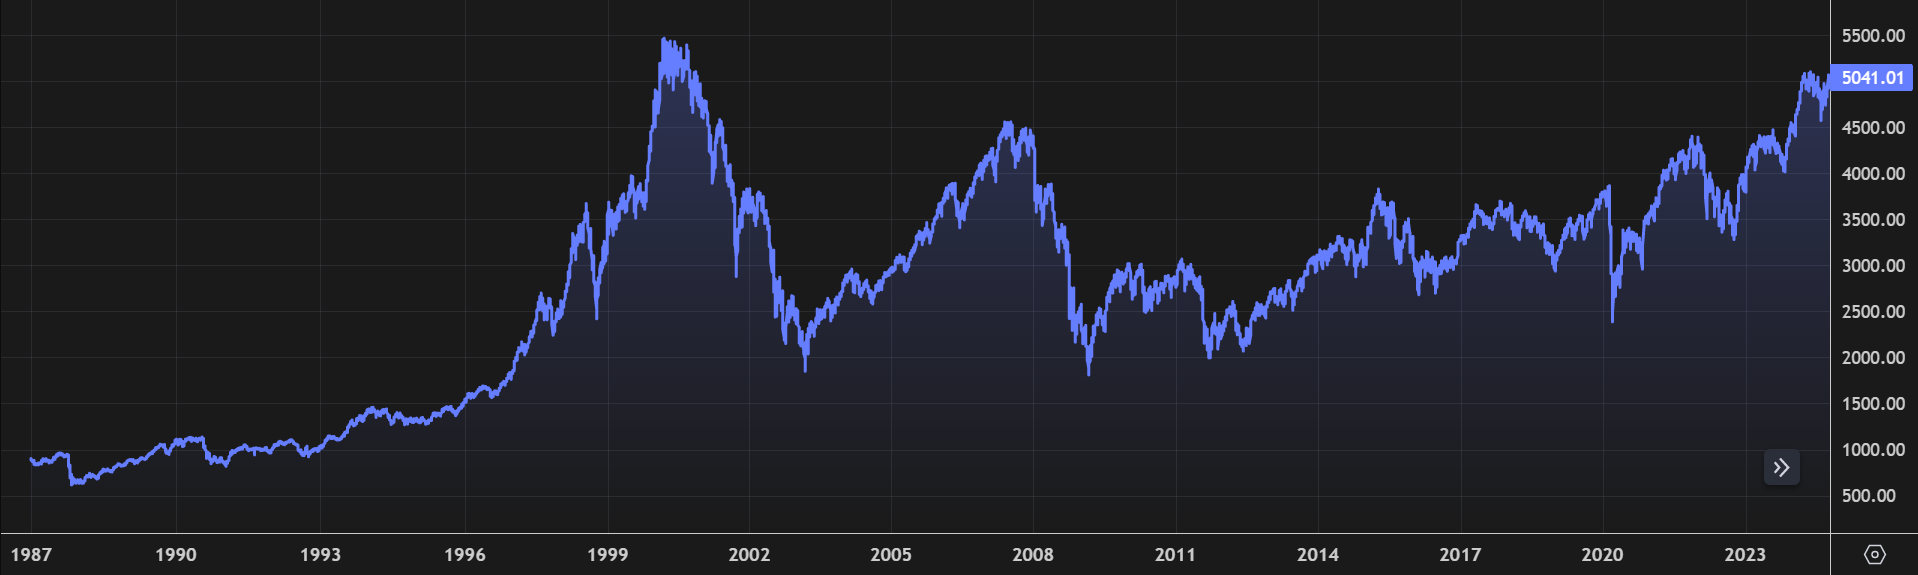
\includegraphics[scale=0.35]{sx5e.png}
    \caption{Euro Stoxx 50 price chart}
\end{figure}

\subsubsection{Brent Crude Oil}
Commodities often have complex dynamics, driven by geopolitical events and natural 
supply and demand. As well as this, oil in particular lends itself to increased
volatility often responding to changes by the Federal Reserve and OPEC(Organisation 
of petroleum-exporting countries). These factors create characteristics such as 
heavy tails and jumps, often not being represented well by traditional models. 
I will be using Brent Oil as a benchmark asset to compare the expressibility of 
quantum derived models vs existing classical ones. 


\subsection{Hedging}
The main issue being tackled in this report is the idea of optimal hedging. 
Hedging itself is the process of mitigating risk through trading other products. 
In this report, I am focussing on hedging an option with an underlying being the 
asset itself. Traditionally hedging involved deriving the exposure to the market, 
after buying an option, using a closed-form solution to classical models. The most 
commonly used is the delta exposure, derived from the Black-Scholes equation. 
The delta of an option is sensitive to the other parameters in BS, the one we're 
most concerned with being the underlying. Delta itself can be thought of as 
$\frac{\partial V}{\partial S}$, the change in the option price with respect to 
the underlying. 
The basic strategy for limiting risk is delta-hedging. This involves analysing 
the combined delta of the options bought and then buying the proportional amount 
in the underlying asset. 
\newp 
The biggest problems with delta-hedging include inaccurate assumptions about the 
underlying's behaviour, only hedging against the delta of the option, and the idea 
of when to hedge. One might take the strategy of hedging whenever the delta of 
the option reaches certain limits, called band-based hedging. This can be done 
efficiently if you are aware of how the option will react for its entire lifetime. 
Unfortunately we don't have such oracles that accurately predict the future, so 
we are left to mathematical assumptions and machine learning techniques to 
model such behaviour. 
\newp 
Deep hedging formulates hedging as a machine learning problem of determining the 
optimal points to hedge an option. Some papers treat this as a reinforcement 
problem, while others rely on time-series analysis. The common theme between 
most models available is the need for an accurate market generator. The underlying 
asset has to be simulated till maturity of the option to determine the best time 
to take a position. For this reason I will be focussing on the accuracy of the 
market generator in the context of deep hedging. 
\clearpage

\section{Merton-Jump Diffusion Model}
My model of choice for comparison is the Merton-Jump Diffusion model, this an 
elementary model that goes beyond Black-Scholes by trying to capture the negative
skewness and excess kurtosis of log price returns. This is done through the 
addition of a compound Poisson jump process. This aims to represent the jumps 
we observe in the market in a more realistic fashion rather than assuming constant 
volatility assumption made by Black-Scholes. As a simplification, I will be referring 
to Black-Scholes by BS and Merton-Jump Diffusion with MJD.
\subsection{Black-Scholes}
Let's start with the Black-Scholes model, an elementary model first proposed in 
1973 by Robert Merton to price European vanilla options. [reference here] \\
Consider a call options on a non-dividend paying stock with expiry T and strike K. 
We will assume that the asset price will obey geometric brownian motion hence 
giving: 
\begin{equation}
dS_t = \mu {S_t} dt + \sigma S_t dW_t
\end{equation}
where $W_t$ is a standard Brownian motion. We assume interest rates to be constant,
meaning a unit of a given currency at time t will be worth $e^{rt}$ at time t.\\
We can now consider the value of our call option $C(S_t,t)$, a twice differentiable 
function of stock price and time, by way of It\^{o}s 
lemma
we can say that 
\begin{equation}
dC = \left( \frac{\partial C}{\partial t} + \mu S \frac{\partial C}{\partial S} + \frac{1}{2} \sigma^2 S^2 \frac{\partial^2 C}{\partial S^2} \right) dt + \sigma S \frac{\partial C}{\partial S} dW
\end{equation}
This is the SDE for the price of an option. In traditional hedging, we would use 
values derived from this SDE to construct a theoretical perfect hedge. 
\subsection{Model}
A standard derivation of the model will allow us to explore its assumptions and 
limitations. This model consists of two components, jump and diffusion. The 
diffusion will be modelled using a Weiner process and log-normal jumps driven 
by a Poisson process. This gives us the following
SDE. 
\begin{equation}
  \italic{d}S_t = (\alpha - \lambda k)S_tdt + \sigma S_t dW_t + (y_t-1)S_tdN_t
\end{equation}
where $W_t \text{ and } N_t$ are Weiner and Poisson processes respectively. 
$\lambda$ represents the intensity of the jumps, $\alpha$ is the drift rate
(expected return), $y_t - 1$ is the relative jump size with $k$ being the mean. 
Solving the equation gives us an exponential L\'{e}vy model described by 
\begin{equation}
  S_t = S_0e^{\mathcal{L}_t}
\end{equation}
where $S_t$ is the stock price at time t, $S_0$ is the initial stock price. 
We can also define $\mathcal{L}_t$ to be 
\begin{equation}
  \mathcal{L}_t = (\alpha - \frac{\sigma^2}{2}-\lambda k)t + \sigma W_t + 
  \sum^{N_t}_{i=1}Y_i
\end{equation}
$\sum_{i=1}^{N_t}Y_i$ being the compound Poisson process. 
\subsection{Assumptions \& Limitations}
Through inspection of the equations, we can observe the following assumptions:
\begin{enumerate}
\item The asset price experiences continuous, random fluctuations over time,
  governed by Brownian motion (GBM)
\item The asset price experiences sudden, discontinuous jumps modelled by a 
  Poisson process, occurring at a constant rate $\lambda$
\item Jumps sizes are assumed to be log-normal $ln(y_t) \sim \mathcal{N}(\mu,\sigma^2)$
\end{enumerate}
Starting with the first assumption, we can see that assuming GBM may produce
unrealistic behaviour, most important being a lack of excess kurtosis.
Markets 
often exhibit fat tails, especially within commodities. One such event may 
be the release of news from OPEC+, the organisation of petroleum-exporting 
countries. A restriction in oil production may cause the price of oil to jump 
rapidly. In recent times, wars and conflict has also become 
ever present, causing large movements in asset prices; therefore it is not 
unrealistic to
expect extreme price movements to be more frequent than can be modelled 
by a Gaussian.
\newp
The MJD requires calibration of parameters before use, typically done using historical 
data or implied volatility surfaces. Once calibrated these become assumptions of 
the data and so do not change even if the market observations move away from it. 
This would lead us to expect higher overfitting to the historical data, possibly 
failing in unseen conditions such as the market's reaction to COVID. 
\newp 
We also may expect poor volatility clustering with the MJD; constant volatility 
is not experienced by the market, instead periods of high volatility followed 
by periods of low volatility is observed. Though this paper won't be focussing 
on this phenomenon, it is important to consider.
\subsection{Calibration}
In this research, I have chosen to use maximum likelihood estimation to estimate 
the parameters for the MJD model. In the analytical solution we require five 
parameters: $\alpha$, $\sigma$, $\mu_j$, $\delta$, and $\lambda$. These are the 
expected return, volatility of the given asset, expectation of the jump size, 
standard deviation of the jump size and lastly the jump intensity. We can then 
use MLE on the probability density of log returns $S_t = ln(\frac{S_t}{S_0})$ 
\begin{equation}
P(S_t) = \sum^\infty_{i=0} \frac{e^{-\lambda t}(\lambda t)^i}{i!}N(S_t;(\alpha - 
\frac{\sigma^2}{2}-\lambda k)t+i\mu_j,\sigma^2t+i\delta^2)
\end{equation}
The likelihood function hence becomes 
\begin{equation}
  L(\theta;S) = \prod^T_{t=1}P(S_t)
\end{equation}
We can minimise the negative log-likelihood to obtain 
\begin{equation}
  -\ln L(\theta;S) = -\sum^T_{t=1}\ln P(S_t)
\end{equation}
Another popular option to calibrate the MJD model is by considering the implied 
volatility surface of existing options. This technique can lead to a 
calibration but suffers with issues surrounding the sensitivity of the tails of 
the asset prices. It is also well documented that given a function that measures 
the calibration error, we can observe a largely flat landscape surrounding the 
optimal solution, 
implying obtaining accurate parameters can become very computationally 
expensive, often requiring hundreds of iterations \autocite{jump05}. These difficulties
can translate into a poor hedge, leaving a buyer overexposed to market fluctuations. 

\clearpage


\section{Quantum Computing}
This section aims to serve as a brief introduction to quantum computing. 
\subsection{Quantum Systems}
Unlike classical computing, quantum computing acts in a non-deterministic manner,
the computer remains in multiple states with given probabilities rather than a
fixed resultant state as expected from classical computers. Formally we can define 
a qubit to be a quantum system where the states of 0 and 1 are represented by a pair 
of normalised and mutually orthogonal quantum states $|0\rangle$ and $|1\rangle$. 
Intuitively however, let's start with a two-state machine; 
we can describe such system to be in the state 
$|0\rangle$ with some amplitude $\alpha$ and in $|1\rangle$ with amplitude $\beta$. 
This can be represented  as
\begin{equation}\label{eq51}
  |\psi\rangle = \alpha|0\rangle + \beta|1\rangle = \alpha\begin{pmatrix} 
    1\\0\end{pmatrix} + \beta\begin{pmatrix}0\\1\end{pmatrix}
\end{equation}
for 
some $\alpha$ and $\beta$ such that $|\alpha|^2+|\beta|^2 = 1$; 
we can refer to this as a superposition of the states $|0\rangle$ and $|1\rangle$. 
If measured in the standard basis, we would expect the outcome to be $|k\rangle$ 
with a certain probability, this outcome resulting in the output state of the 
measurement gate to also be $|k\rangle$. This would mean our initial state $|\psi\rangle$
is irreversibly lost; we refer to this as a collapse of state.
\newp 
Each qubit can 
be thought of as a vector, $\bold{v}$, on a Bloch's sphere which can be represented in two 
basis: $\theta$ and $\varphi$. $\theta$ is the angle between $\bold{v}$ and the 
z-axis. $\varphi$ becomes the angle between $\bold{v}$ and the x-axis. Considering 
a more general parameterisation of 
\ref{eq51} gives us 
\begin{equation}\label{hilbert1}
  |\psi\rangle = \cos (\frac{\theta}{2})|0\rangle + \sin(\frac{\theta}
  {2})e^{i\varphi}|1\rangle
\end{equation}
\begin{figure}[h!]
  \centering 
  \includegraphics[width=\linewidth]{blochsphere.jpg}
  \caption{Bloch sphere}
  \label{fig:bloch}
\end{figure}
\newp 
\subsubsection{Tensor Products}
Tensor products, $\otimes$, to allow us to combine vector spaces. Lets consider 
a two qubit system:
\begin{equation}
  |\psi\rangle = \alpha_0|0\rangle + \alpha_1|1\rangle \text{  and  }
  |\phi\rangle = \beta_0|1\rangle  + \beta_1|1\rangle
\end{equation}
their tensor product becomes:
\begin{equation}
  |\psi\rangle \otimes |\phi\rangle = 
  \alpha_0\beta_0|00\rangle + 
  \alpha_0\beta_1|01\rangle + 
  \alpha_1\beta_0|10\rangle + 
  \alpha_1\beta_1|11\rangle  
\end{equation}
\subsubsection{N-qubit systems}
The Bloch sphere, figure \ref{fig:bloch}, allows us to visualise all the pure states and the rotations taken 
on $\bold{v}$. 
The space of all the possible orientations of $\psi$ is called the Hilbert space. 
Formally a Hilbert space, $\mathcal{H}$, is a vector space which is an inner product space 
over $\mathcal{C}$ that is also complete with respect to the norm. For a single 
qubit the state space is $\mathbb{C}^2$, a 2-dimensional Hilbert space, satisfying 
\ref{hilbert1}. When extending to n qubits, the Hilbert space becomes 
\begin{equation}
  \mathcal{H}_n = \mathbb{C}^2 \otimes \mathbb{C}^2 \otimes ... \otimes \mathbb{C}^2 
  =(\mathbb{C}^2)^{\otimes n} = \mathbb{C}^{2^n}
\end{equation}
The computational basis for $\mathcal{H}_n$ consists of all the possible n-bit strings:
\begin{equation}
  \{|x_1x_2...x_n\rangle\}, \text{ where } x_i \in \{0,1\}
\end{equation}
There are $2^n$ such basis states, each representing a classical bit string\\
(e.g. $|00...0\rangle$,$|00...1\rangle$,...,$|11...1|\rangle$). 

\subsubsection{Entanglement}
Quantum entanglement is a fundamental feature of quantum mechanics, allowing 
qubits to be deeply correlated to the point their joint state cannot be represented 
as a product of their individual states. Measurement of one state will have an 
instantaneous impact on the other entangled qubit, determining the outcome for both 
qubits. 
Entanglement emerges from the structure of the tensor product. A state 
$|\psi\rangle \in \mathbb{C}^2 \otimes \mathbb{C}^2$ is entangled if there are 
correlations between measurement outcomes of each qubit that cannot be explained
by any product of the independent states, we cannot decompose it into 
$|\psi\rangle = |\psi_A\rangle \otimes |\psi_B\rangle$ for some $\psi_A \in \mathcal{H}_A$
and $|\psi_B\rangle \in \mathcal{H}_B$.


\newp
\subsection{Quantum Operators}
Before forming quantum circuits, we must first understand how quantum gates operate. 
In quantum computing, the evolution of quantum states is governed by unitary 
operations, linear transformations $U: \mathcal{H} \rightarrow \mathcal{H}$ satisfying 
$U^{\dagger}U = UU^{\dagger} = I$. These are implemented as quantum gates, acting on 
the qubits with single-qubit gates being represented by $2\times2$ unitary matrices,
and multi-qubit by tensor products. There are many gates but the ones we will 
discuss the ones used in this project. 
\newp
The Pauli group is a foundational set of operators that consists of three Pauli 
matrices and an identity. These form an orthonormal basis for $2\times 2$ Hermitian 
matrices, $P=P^{\dagger}$ where $P^{\dagger}$ is the conjugate transpose, and are 
crucial for in defining measurements, quantum error correction, and stabiliser 
circuits. For a single qubit, we can define the Pauli group, $\mathcal{P}$, with 
phases $\{\pm1, \pm i\}$ to be 
\begin{equation}
  \mathcal{P} = \{\pm I, \pm iI, \pm X, \pm iX, \pm Y, \pm iY, \pm Z, \pm iZ\}
\end{equation}
where
\begin{equation}
X = \begin{pmatrix} 0 & 1 \\ 1 & 0 \end{pmatrix}, \quad
Y = \begin{pmatrix} 0 & -i \\ i & 0 \end{pmatrix}, \quad
Z = \begin{pmatrix} 1 & 0 \\ 0 & -1 \end{pmatrix}, \quad
I = \begin{pmatrix} 1 & 0 \\ 0 & 1 \end{pmatrix} \quad
\end{equation}
\newp 
We can extend this to the Pauli rotation gates which 
allow you to rotate a vector around the Bloch sphere. The first one, $R_x(\theta)$,
allows us to rotate a qubit around the x-axis and is given by:
$$
R_x(\theta)& = \coloneqq 
\begin{bmatrix}
\cos(\theta/2) & -i\sin(\theta/2) \\
-i\sin(\theta/2) & \cos(\theta/2)
\end{bmatrix}
$$ 
Likewise the $R_y$ and $R_z$ are defined similarly, allowing rotations around the 
y and z axes.
$$
R_y(\theta) = \coloneqq 
\begin{bmatrix}
\cos(\theta/2) & -\sin(\theta/2) \\
\sin(\theta/2) & \cos(\theta/2)
\end{bmatrix}
$$
$$
R_z(\theta) = \coloneqq 
\begin{bmatrix}
e^{-i\theta/2} & 0 \\
0 & e^{i\theta/2}
\end{bmatrix}
$$
It is worth noticing the Pauli X gate is equivalent to a rotation of $\pi$ in the 
x-axis, which can also be represented as $R_x(\pi)$. 
Another key gate is the CNOT gate, a two-qubit gate used to generate entanglement. 
The CNOT acts on a control and target qubit, flipping the target if the control 
qubit is in the $|1\rangle$ state. 
$$
CNOT =
\begin{pmatrix}
1 & 0 & 0 & 0 \\
0 & 1 & 0 & 0 \\
0 & 0 & 0 & 1 \\
0 & 0 & 1 & 0
\end{pmatrix}
$$
These entangled states are crucial for learning complex distributions, allowing us 
to faithfully create synthetic market data. 
\subsection{Clifford and non-Clifford Gates}
Often articles focus on the benefits of quantum computing being superposition 
and entanglement but we can think beyond that and consider those gates that can't
be efficiently simulated classically, the untold heroes. 
The operations we have discussed previously such as Pauli $X$, $CNOT$ etc. can be put 
into two main categories: Clifford and non-Clifford. The Clifford group involves 
those gates that can be simulated efficiently classically, with non-Clifford 
containing those that are responsible for the quantum speed ups observed such as 
the T-gates. 
\newp 
Clifford group contains those gates that map Pauli operators to other Pauli 
operators under conjugation. We can formally say that for a Clifford unitary, $U$, 
and for every Pauli operator, $P$, $UPU^{\dagger}$ is still a Pauli operator. 
These, however, do not form a universal set of quantum gates so require 
non-Clifford operators. Though not able to represent every possible operation,
they still serve a large purpose, typically being used in quantum error correction 
algorithms or for testing entanglement. 
\newp 
Non-Clifford gates are those that cannot be simulated efficiently on a classical 
machine, a common being the T-gate. 
\begin{equation}
  T = 
  \begin{pmatrix} 
1 & 0 \\ 
0 & e^{i\pi/4} 
\end{pmatrix} 
\end{equation}
An important property that defines this as non-Clifford is the fact that is doesn't 
preserve the Pauli group under conjugation. Formally 
\begin{equation}
  TXT^{\dagger} \neq \text{Pauli Operator}
\end{equation}
Another important gate is the Toffoli gate which serves as a three-qubit gate 
that applies a NOT operation the third qubit if the first two qubits are in the 
$|1\rangle$ state.
\newp 
Non-Clifford gates can be non-trivial to implement unfortunately. 
One such method for implementation of non-Cliffords includes magic state 
distillation, using ancilla bits to aid the computation, adding large computational 
costs. These also often require non-transversal methods which can increase the 
error propagation, making a fault tolerant device ever more difficult. For this 
reason, we would like a framework to reduce the T-gate count in a circuit.

\subsection{Born Rule}
An essential part of quantum computing involves the existence of the Born
Rule. Given a quantum state $|\psi\rangle \in \mathcal{H}$, the Born rule states 
the probability of measuring an outcome $x \in \{0,1\}^n$ in the computational 
basis is
\begin{equation}
p(x) = |\langle x|\psi(\theta)\rangle|^2
\end{equation} where 
\begin{equation}
|\psi(\theta)\rangle = U(\theta)|0\rangle^{\otimes n}
\end{equation}
This means that the probability distribution over all possible $2^n$ outcomes 
is derived from the squared magnitudes of the amplitudes in the quantum state 
vector. Unlike classical probabilistic models, where probabilities are assigned 
directly, quantum probabilities arise from the inner product between the quantum 
and measurement state, through the application of the Born rule. As such, the 
quantum devices are able to leverage superposition and interference effects that 
have no classical counterpart. This makes it suitable for representing probability 
distributions with non-trivial structures such as financial time-series with jumps, 
or fat-tailed behaviours.
\newp
LOOK INTO CHANGING:\\
The state $|\psi(\theta)\rangle$ is generated by evolving state $|0\rangle$
according to a Hamiltonian $H$ that is constructed from gates. Once combined, the 
gates form a parameterised quantum circuit which is parameterised by using the 
variables governing each gate, $\theta$. By tuning the values of $\theta_i$ one 
can allow for an evolution to any state that will serve as a solution to a given 
problem. \\ 
By taking the distribution associated to the state, $|\psi(\theta)\rangle$ we can 
treat the PQC as a generative model, upon measurement will 
generate samples of a target distribution $\chi$. This model is parameterised 
by $\theta$, which defines a quantum circuit $U(\theta)$ made up of a set of quantum 
gates.
By measuring the circuit, we can obtain samples. Producing samples that emulate 
the target distribution involves minimising the parameters of the circuit $U(\theta)$, 
a process once convergence is reached, will generate accurate samples 
\cite{liu_differentiable_2018}.


\subsection{Parameterised Quantum Circuits}
Parameterised quantum circuits(PQCs) are a powerful framework consisting of rotation 
and entanglement gates for hybrid quantum-classical algorithms. A PQC is a quantum 
circuit with rotation gates with parameters $\theta = (\theta_1, \theta_2...\theta_n)$
which can be tuned classically to give desired results. These rotations are often 
interleaved with entanglement gates such as CNOTs. The design of the PQC is 
dependant on the choice of ansatz used; an ansatz can be thought of as a trial 
state that is used as the starting point 
for the optimisations. It's an empty canvas with gates and parameters that need 
to be tuned to give meaning.
\newp 
When thinking about PQCs, we must also discuss NISQ(Noisy Intermediate-Scale 
Quantum) devices. These are the current generation of quantum processors that 
have limited qubit counts, roughly 1000 qubits, but lack quantum error correction; 
this makes them prone to noise and decoherence. This makes the devices very sensitive 
to external interference, especially from the environment. These computers aim 
to serve as a vehicle for research rather than providing a quantum advantage 
at this time.
\newp
The biggest challenge of NISQ devices is the high error rates which may render 
quantum algorithms useless due to the volume of noise. Noise can significantly 
worsen the barren plateau effect, expanded on further in this report, flattening 
the optimisation landscape. If the noise grows, it can have the effect of acting 
as random unitary operation, possibly causing gradients to vanish or making it 
difficult for classical optimisers to understand descent directions. 
Due to this, it is imperative to keep gate and entanglement counts to the acceptable 
minimum. This gives way to research on optimal circuits; I have tried to investigate 
the effect of the circuit ansatz on the end result, showing slight modifications 
to entanglement structures can have a large effect on the trainability and 
expressibility. 

\subsection{Basis Encoding}
When modelled data is drawn from a continuous domain, log returns, the output 
space must be discretized to be representable in the computational basis. We 
achieve this through the process of basis encoding, involving binning the 
input data. Formally, given a continuous random variable, $X \in \mathbb{R}$, 
we discretize this into $2^n$ bins, where each bin corresponds to a 
basis state $|x\rangle$ for $x \in \{0,1\}^n$.
This encoding induces a discrete probability distribution over the basis states 
which becomes the empirical target distribution for the training the quantum circuit;
 the PQC can then learn to approximate this histogram-like distribution using the 
Born rule.
It is important to note that the resolution of the learnt distribution is therefore 
limited by the number of qubits, $n$, so should be a consideration when designing 
the PQC. 
\newp 
This process allows us to use classical statistical divergences such as Kullback-Leibler 
divergence for loss function since both the model and data reside in a common 
discrete sample space. 
\newpage
\section{Quantum Circuit Born Machine}
The Quantum Circuit Born Machine(QCBM) is an extension of PQCs, designed with the 
intent of probabilistic generation at its core. It consists of a PQC with trainable 
parameters, $\theta$. These parameters can be tuned through an optimisation process 
such that sampling the PQC replicates a target distribution. This is the model that 
is leveraged to generate the synthetic market data.
\newp
Formally, given a dataset $D = \{x_1, x_2.. x_n\}$ consisting of $n$ market observations and 
obeys a given distribution $\chi_d$, we would like the QCBM to replicate the distribution 
and, once sampled, generate synthetic data points that are of the distribution $\chi_s$ 
such that $\chi_s$ approximates $\chi_d$.
\newp
Let $U(\theta)$ be a PQC acting on $n$ qubits, where $\theta \in \mathcal{R}^m$ 
is a vector of tunable parameters. Initially, the circuit will prepare a quantum 
state:
\begin{equation}
|\psi(\theta)\rangle = U(\theta)|0\rangle^{\otimes n}
\end{equation}
$|0\rangle^{\otimes n}$ representing all the qubits in the computational basis
state $|0\rangle$.\\
Upon measurement in the computational basis, this state will produce a probability 
distribution according to Born's rule: 
\begin{equation}
p_{\theta}(x) = |\langle x|\psi(\theta)\rangle|^2
\end{equation}
where $x\in\{0,1\}^n$ represents a bit string of measurement outcomes. The goal 
of the QCBM now becomes to find optimal parameters of $\theta$ such that the 
output probability distribution replicates that of the target, letting $p_{\theta}
(x)$ approach $\chi_d$.
\subsection{Implementation}
The distribution to be learnt could not simply be the price at each time stamp, 
as sampling the QCBM would remove any time component associated. Many ideas were tested 
but the final design involved learning the distribution of log returns. This was 
acceptable as we would be simulating many paths and less focussed on the given 
price at each point. Formally, we are learning $r$, the log returns, and propagating 
the series using 
\begin{equation}
  S_t = S_{t-1}e^{r_t}
\end{equation}
At each time step, the QCBM is sampled to gain a log return to be used to generate 
the next value. Limitations of this can involve lack of volatility clustering which 
can make it unsuitable for time-series prediction, though uses a similar technique 
to classical methods. In the results section I explore whether this method does 
provide a better hedge or not.
\newp
Implementation of the QCBM involved a few more steps. The target distribution 
is of log returns, so the market data had to be converted into the appropriate 
format. Before using the QCBM, the input data must also be discretised. This 
involves binning the log returns into $2^n$ bins, where $n$ is the number of 
qubits in the system. The value of $n$ is chosen based on the accuracy desired, 
with larger values of $n$ allowing for more 'bins', leading to better expressibility.
Making $n$ too large can lead to issues with optimisation and giving way to the 
barren plateau phenomenon.
\newp
The training process then involves minimising a loss function, in this case using 
the Kullback-Leibler(KL) Divergence. 
\begin{equation}
\mathcal{L}_{KL}(\theta) = \sum_{x \in \{0,1\}^n}q(x)log\bigl( \frac{q(x)}{p_{\theta(x)}}\bigr)
\end{equation}
Optimisation of these parameters was left to the PennyLane[ref here] package. 
The optimiser chosen is Adam, a gradient-descent optimiser with adaptive 
learning rates.
\newp
The ansatz for this quantum circuit was varied, testing multiple architectures
to explore the effects, expanded on further in section 6.2.
\newp
The final pipeline for the QCBM is as follows:
\begin{enumerate}
  \item Pre-processing of market data
  \item Binning/discretising the input data
  \item Constructing the PQC for the QCBM
  \item Comparison of QCBM's probability distribution to target distribution using
  KL Divergence
  \item Optimisation of QCBM's parameters, $\theta$
  \item Analysis of synthetic distribution
\end{enumerate}

\begin{figure}[h!]
  \centering 
  \includegraphics[scale=0.32]{Overview.png}
  \caption{Overview of the QCBM design}
  \label{fig:overview}
\end{figure}

\newpage
\subsection{Barren Plateau}
A point of concern when searching for the optimal set of $\theta s$ is the large 
search space, here we may observe issues such as barren plateau(BP). BP 
insists that the gradient of the parameters of a given PQC will vanish exponentially 
with respect to the search space. McClean[ref here] shows that for a PQC with $L$ layers in the form: 
\begin{equation}
  U(\theta) = \Pi_L^{l=1}U_l(\theta_l)W_l
\end{equation}
where $U_l(\theta_l)$ are parameterised gates and $W_l$ are fixed gates, and with 
cost function:
\begin{equation}
E(\theta) = \bra{0}U(\theta)^\dagger HU(\theta)\ket{0}
\end{equation}
where $H$ is a Hermitian observable, the gradient variance vanishes exponentially,
leaving us with the following relationship:
\begin{equation}
  Var[\partial_kC(\theta)] \leq \mathcal{O}\bigl(\frac{1}{2n}\bigr)
\end{equation}
for n-qubits. 
\newp 
This shows us to expect flat optimisation landscapes, leading to sub-optimal values
of $\theta$ being learnt. This relationship also shows us why the ansatz chosen 
makes a big difference on the learnability, something I further explore in the 
next section. 
\subsection{Architectures}
The design of the ansatz can significantly affect the ability to learn and represent 
the target distribution. The number of gates, depth, and entanglement structure
all affect the expressibility and trainability of the circuit. Circuits with 
higher entanglement and parameterised gates are theoretically able to represent 
any distribution, though it comes at the cost of noise and barren plateaus. 
Choosing a simpler ansatz may converge quicker but results in a weaker approximation,
oversimplifying the solution.
The architecture will also affect the optimisation landscape; random parameterised 
circuits with deep, unstructured layers are more prone to barren plateaus, making 
training very difficult. Due to this we strive for a balance, one that is 
able to learn the complexities of the market without compromising on finding the 
optimal parameters.
\subsubsection{Brick}
The first architecture investigated is the Brick architecture. This ansatz arranges
the gates in a staggered, layered pattern that resembles a brick wall. These 
have alternating layers of single-qubit rotation and nearest-neighbour hardware
connectivity. This simple
entanglement structure provided the best trainability, converging to a solution 
much faster than the other circuits. We can argue this was the case due to 
their local connectivity, on NISQ devices it is able to minimise cumulative 
errors. 
As well as this, the KL divergence loss was 
often much lower than the other circuits. For these reasons it was the circuit 
of choice for all the results in the following sections.
\newp 
It must be said that research indicates this structure can face scaling limitations 
for problems that require long-range correlations. In the paper we are investigating 
correlations between 2 prices so are not affected by this property but it should 
be noted for any further developments made beyond this report. [ref:  Empirical Comparisons on NISQ Devices]. 

\begin{figure}[h!]
  \centering 
  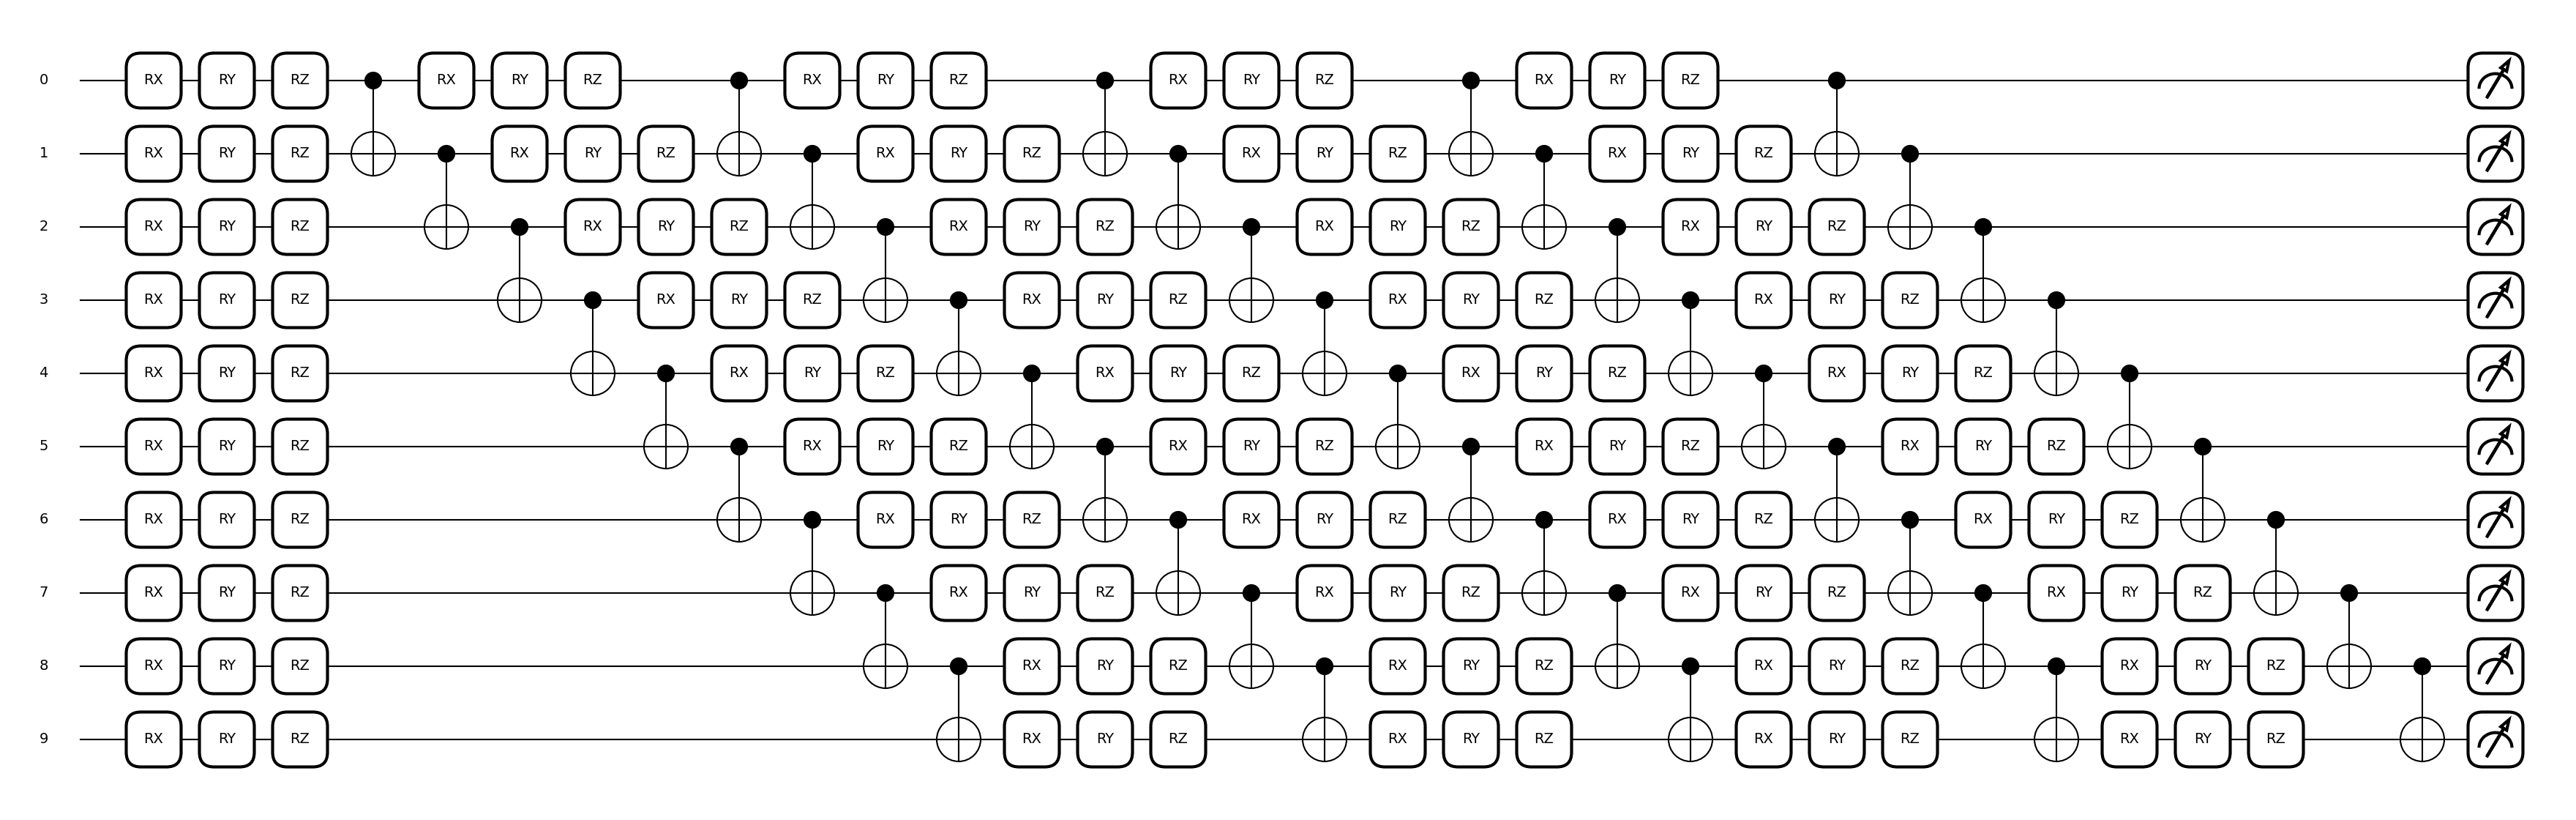
\includegraphics[width=\linewidth]{ten5brick.png}
  \caption{10x5 Brick Ansatz}
  \label{fig:brick}
\end{figure}

\subsubsection{Pyramid}
Though shown that the Brick ansatz provides the best results, it is important to 
test other circuits as well. The pyramid structure offers a simpler entanglement 
structure compared to the brick, also having nearest-neighbour hardware 
connectivity. This made trainability less of a concern but 
when looking at the KL divergence, it offered a worse loss indicating the 
easier optimisation came at the cost of expressibility. We could make conclusions 
that this circuit was not able to learn the appropriate correlations in the data,
making it less effective than a traditional model. 
\begin{figure}[h!]
  \centering 
  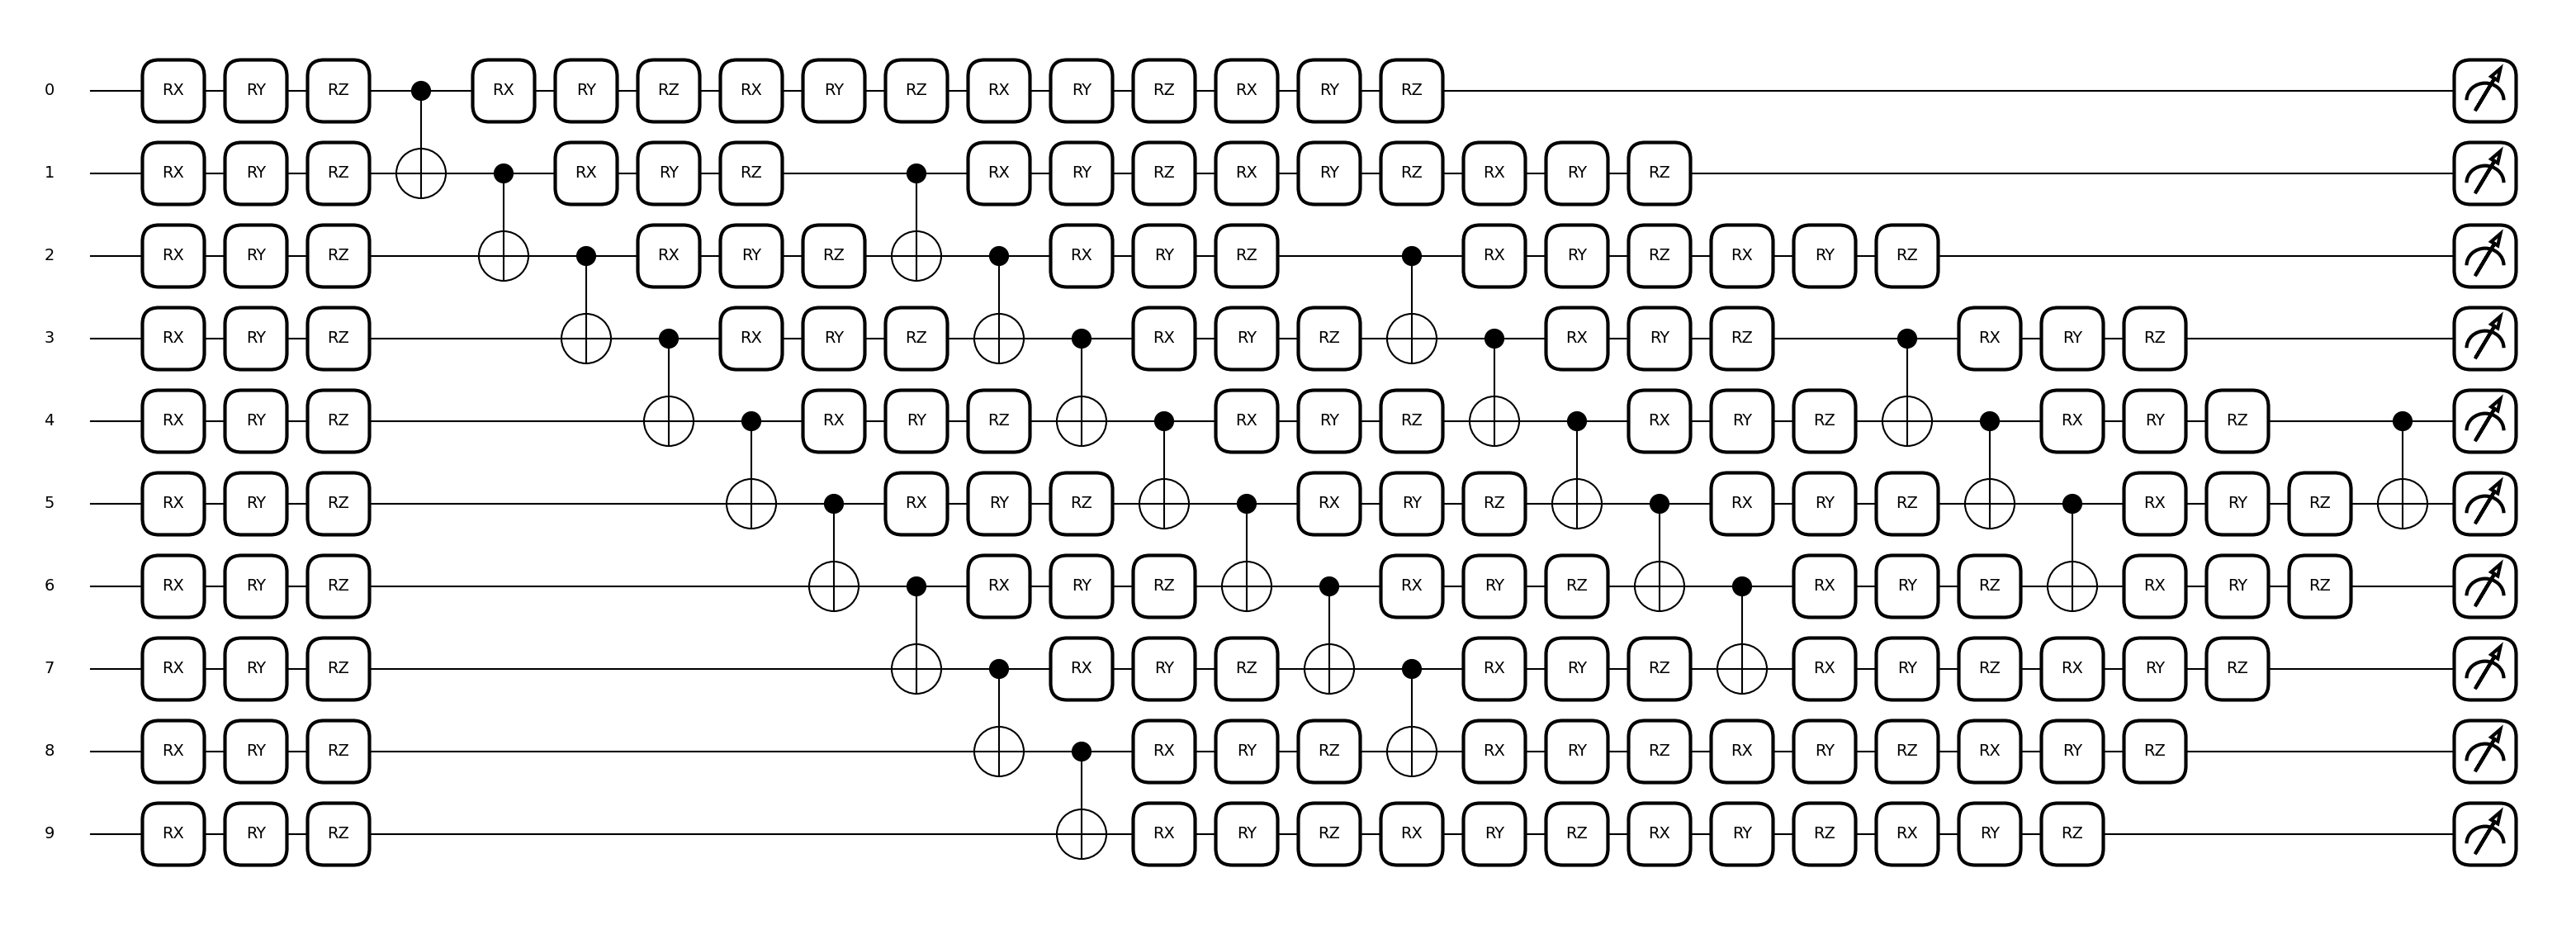
\includegraphics[width=\linewidth]{ten5pyramid.png}
  \caption{10x5 Pyramid Ansatz}
  \label{fig:pyramid}
\end{figure}

\newpage
\subsubsection{Butterfly}
The Butterfly offers a more complex entanglement structure, with all-to-all hardware 
connectivity. This theoretically should provide less gate overhead but physical 
implementations experience practical issues. The physical wiring for all-to-all 
can prove to be a complex problem. The increased wiring between all the qubits 
can lead to higher likelihood of crosstalk and noise creating unwanted interactions 
between qubits. This further relies on better error correction algorithms. Though 
this paper focusses on a theoretical implementation on a quantum simulator, it 
is still necessary to consider practical implications with NISQ devices. 
\newp
This architecture provided worse results than the Brick ansatz, often getting 
stuck at a far higher loss. This implies a difficult loss landscape and the 
implication of barren plateau. These issue made it unsuitable for use. 
[ref: https://arxiv.org/pdf/2209.08167]
\begin{figure}[h!]
  \centering 
  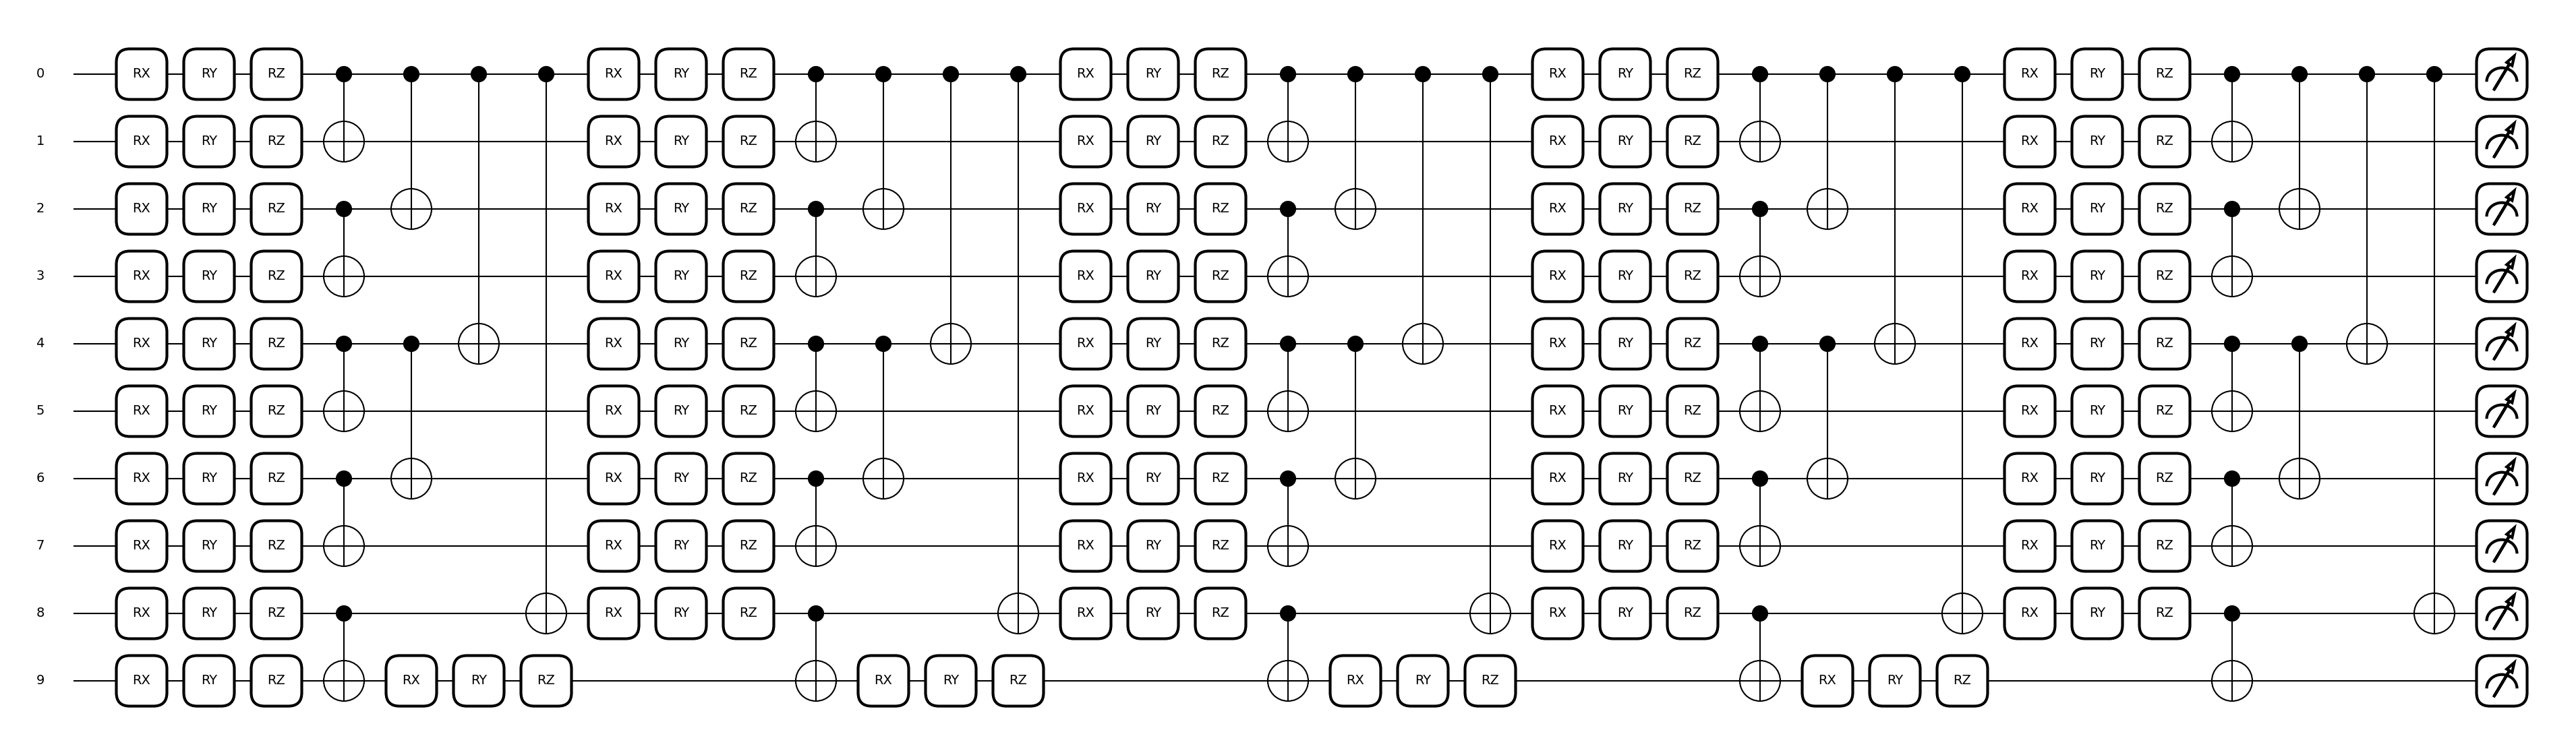
\includegraphics[width=\linewidth]{ten5butterfly.png}
  \caption{10x5 Butterfly Ansatz}
  \label{fig:butterfly}
\end{figure}
\newpage



\subsection{ZX Calculus}
ZX Calculus is a graphical language designed to express the relationships between 
qubits based on category theory. Instead of thinking about the linear maps taking place
in the form of matrices, we can reason about it in a diagrammatic way. This 
can make analysing quantum processes easier and more intuitive. This approach 
makes identifying circuit equalities easier, rather than working out the resultant 
matrix operation for two given circuits. ZX calculus represents the quantum states 
and maps as 'spiders' and 'wires'. 
\newp 
At the heart of ZX calculus are two types of generators: Z-spiders and X-spiders,
represented by green and red nodes respectively. First looking at the Z-spider: 
\begin{equation}
  Z^n_m[\alpha] = |0\rangle^{\otimes n}\langle0|^{\otimes m}+e^{i\alpha}
  |1\rangle^{\otimes n}\langle1|^{\otimes m}
\end{equation}
where m is the number of inputs, n is the number of outputs and $\alpha$ is the 
phase.
\newp
X-spiders are similar to Z-spiders but everything is defined in the X-basis rather 
than the Z-basis. 
\begin{equation}
  X^n_m[\alpha] = |+\rangle^{\otimes n}\langle +|^{\otimes m}+e^{i\alpha}| -\rangle 
  ^{\otimes n}\langle - | ^{\otimes m}
\end{equation}
Thinking about the X-spiders in the Z-basis gives us the following: 
\begin{equation}
  \begin{split}
    |+\rangle &= \frac{1}{\sqrt2}(|0\rangle+|1\rangle)\\
    |-\rangle &= \frac{1}{\sqrt2}(|0\rangle-|1\rangle)
  \end{split}
\end{equation}
and by symmetry
\begin{equation}
  \begin{split}
    |0\rangle &= \frac{1}{\sqrt2}(|+\rangle+|-\rangle)\\
    |1\rangle &= \frac{1}{\sqrt2}(|+\rangle-|-\rangle)
  \end{split}
\end{equation}
The graphical rules of ZX calculus allow for spider fusions, copying and wire 
transformations, all that correspond to those from category theory. It is crucial 
to note/ that ZX calculus is universal for quantum computations, so any computation 
to exist can be represented and reasoned about within this framework. 
\subsubsection{Gate Optimisation}
As mentioned above, non-Clifford gates can be very computationally intensive to 
implement, therefore we would like to reduce any T-gates that don't need to be 
in the circuit. 
\newp 
ZX calculus provides us with a framework to optimise the T-gate count by a process
referred to as gadgetisation. This involves splitting a non-Clifford node into a 
node of itself and a 'phase gadget',a phase that can explore the ZX diagram in 
search of combination or cancellation.[ref here] The ZX diagrams can then be converted back 
into a quantum circuit with potentially less non-Clifford gates. This optimisation 
is implemented in the Python PyZX package[ref here]. I explore the effects of this 
further in the results section.
\newpage
\section{Results}
Putting the theory into practice offered insights into the strengths and weaknesses 
of the model. This section aims to provide quantitative comparisons between the 
classical and quantum methods. After careful consideration and analysis of parameters 
for the QCBM, the model used for comparisons against the MJD model is a 13 qubit,
7 layer model. It uses the brick architecture and has been trained for 500 epochs 
with an Adam optimiser. 
\subsection{Path Generation}
An important part of risk analysis involves path generation, simulating an equity 
path for the next $n$ days. This provides a range of final values, aiming to 
simulate price paths accurately in the process. The metrics involved in the analysis 
involves comparing: the skewness, excess kurtosis, and standard deviation. 
For a return $r_i$ and mean return $\bar{r}$ 
\\Standard deviation:
$$
\sigma = \sqrt{\frac{1}{N} \sum_{i=1}^{N} (r_i - \bar{r})^2}
$$
Skewness:
$$
\gamma_1 = \frac{\sum_{i=1}^{N} (r_i - \bar{r})^3}{(N-1) \times \sigma^3}
$$

Excess kurtosis:
$$
\gamma_2 = \frac{1}{N}\frac{\sum_{i=1}^{N} (r_i - \bar{r})^4}{\sigma^4} - 3
$$
These 
were chosen to highlight the accuracy of the models as well as the ability to represent 
subtleties in the data such as the asymmetric nature and fat tails that are often 
present in market data. Both models were first calibrated on Brent Crude Oil stock 
prices. The test period combines the training and unseen data to see how well the 
model is able to perform on out-of-sample prices. The period of data includes the 
recent reaction to Trump's tariffs, April 2025. This was included purposely to observe 
the model's resilience to tough market activity and heightened volatility.
\begin{table}[h!]
\centering
\begin{tabular}{|l|c|}
\hline
\textbf{Parameter} & \textbf{Value} \\
\hline
Drift ($\mu$) & 0.37956244 \\
Volatility ($\sigma$) & 0.40736202 \\
Jump Intensity ($\lambda$) & 530.63931692 \\
Jump Mean ($\mu_J$) & -0.00374471 \\
Jump Variance ($\sigma_J^2$) & 0.00065703 \\
\hline
\end{tabular}
\caption{Calibrated Parameters of the MJD Model for Brent Crude Oil}
\label{tab:mjd_params}
\end{table}

\begin{table}[h!]
\centering
\begin{tabular}{lccccc}
\hline
\textbf{} & \textbf{Original Data} & \textbf{Test Data} & \textbf{MJD Data} & \textbf{QCBM Data} \\
\hline 
Standard Deviation & 0.0233 &0.0225 & 0.02647 & 0.0268   \\
Skewness            & 0.6550 &0.6709 & -0.2579 & 0.6215 \\
Excess Kurtosis     & 8.5986 &8.8553 & 7.4809 & 8.7375  \\
\hline
\end{tabular}
\caption{Comparison of Brent data with MJD and QCBM Data}
\label{tab:brentdata}
\end{table}


\begin{table}[h!]
\centering
\begin{tabular}{lcccc}
\hline
\textbf{} & \textbf{Original Data} & \textbf{Test Data} & \textbf{MJD Data} & \textbf{QCBM Data} \\
\hline 
Standard Deviation  & 0.0120  & 0.0270  & 0.0126  & 0.0124 \\
Skewness            & 0.8602  & 1.1640  & -0.2015 & 0.7451 \\
Excess Kurtosis     & 11.5700 & 5.6518  & 11.4330 & 11.3780 \\
\hline
\end{tabular}
\caption{Comparison of Eurexx Data with MJD and QCBM Data}
\label{tab:eurexxdata}
\end{table}



As shown in table \ref{tab:brentdata}, the results highlighted that on training data 
for Brent Crude Oil, the 
MJD model was able to capture the standard deviation better, however the skewness 
and excess kurtosis was represented weakly. This is where the QCBM was able to 
demonstrate superiority, 
capturing the skewness and excess kurtosis with greater accuracy.
\newp 
Table \ref{tab:eurexxdata} supports most of the arguments made, though has shown 
slight superiority in representing the fat tails during the training period. 
As the Eurexx data contains less extreme jumps, we can see the MJD model perform 
better. That being said, we can still observe the skewness being learnt poorly
by the classical model. The test data chosen is a continuation of the training data,
both models showing clear difficulties in generalisation. This can be excused however 
as the metrics differ hugely from the training data. This does raise a point of 
concern whether these methods employed of market behaviour prediction are 
appropriate. For this reason, it is more appropriate to treat the models as a 
synthetic market generator rather than for the purposes of prediction. The differences 
in the MJD performance should be noted, highlighting how classical methods 
tend to struggle in tougher market conditions; this is will be further investigated 
in the following sections.
\begin{figure}[h!]
    \centering
    \begin{minipage}{0.48\textwidth}
        \centering
        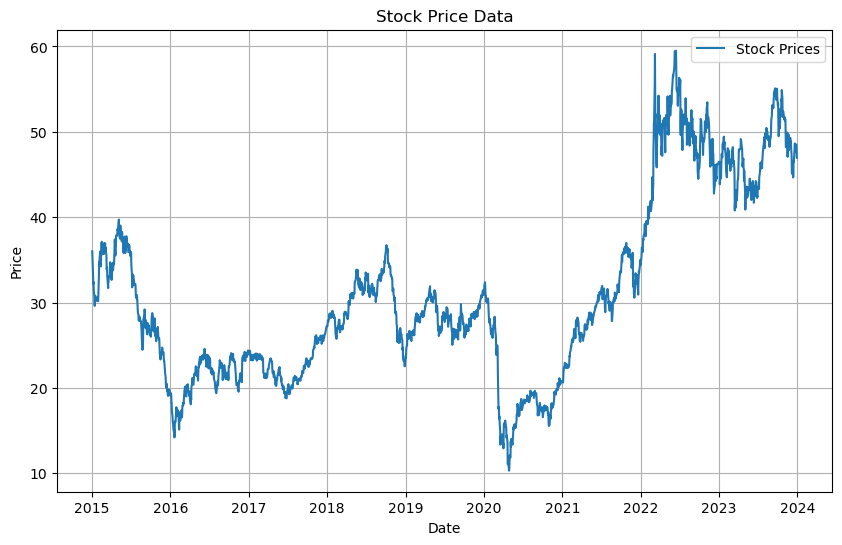
\includegraphics[width=\linewidth]{realpricepath.png}
        \caption{True price path}
        \label{fig:realpricepath}
    \end{minipage}
    \hfill
    \begin{minipage}{0.48\textwidth}
        \centering
        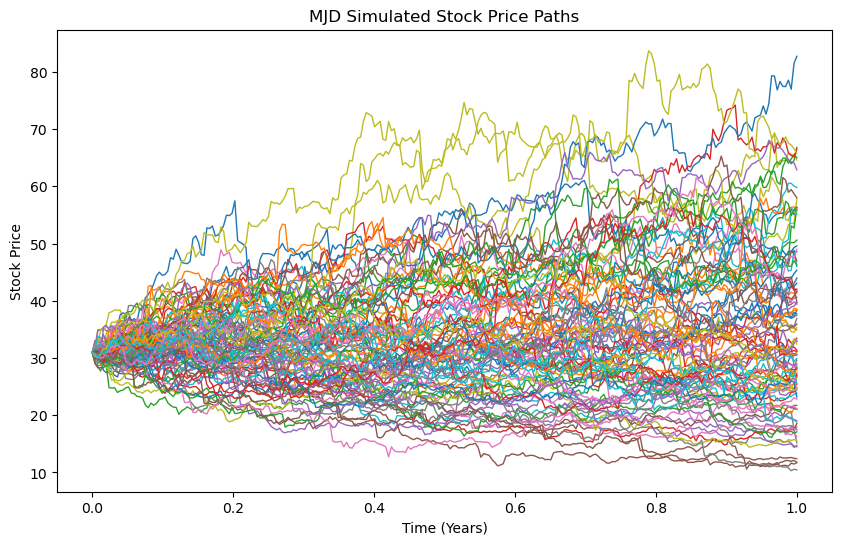
\includegraphics[width=\linewidth]{mjdpricepath.png}
        \caption{Price trajectories for MJD model}
        \label{fig:mjdpricepath}
    \end{minipage}
\end{figure}

\begin{figure}[h!]
    \centering
    \begin{minipage}{0.48\textwidth}
        \centering
        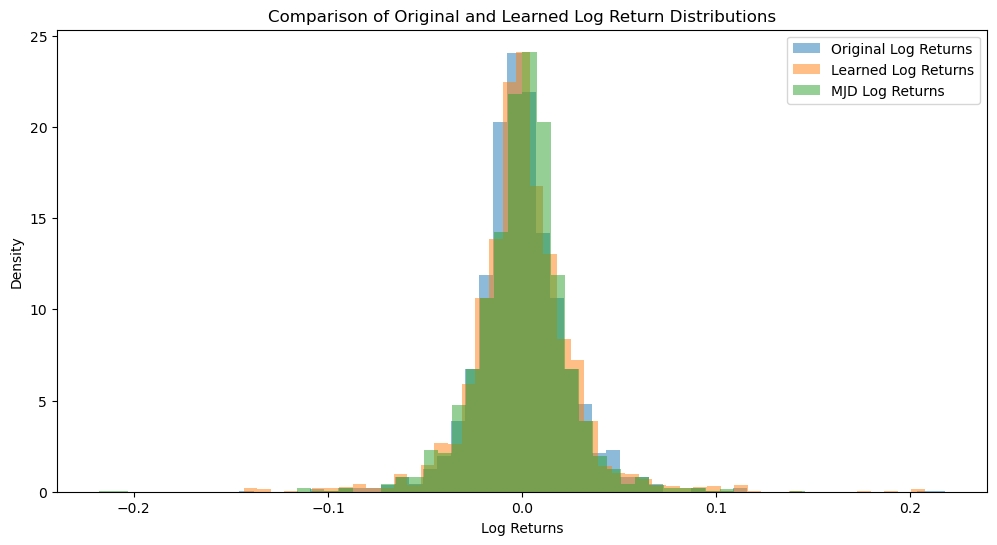
\includegraphics[width=\linewidth]{compdists.png}
        \caption{Comparison of distributions}
        \label{fig:compdists}
    \end{minipage}
    \hfill
    \begin{minipage}{0.48\textwidth}
        \centering
        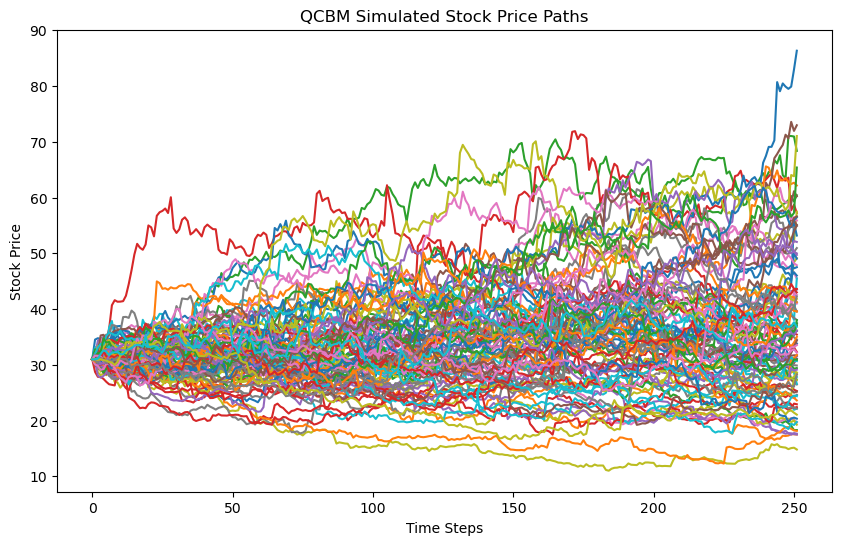
\includegraphics[width=\linewidth]{pricepath2.png}
        \caption{Price trajectories for QCBM model}
        \label{fig:pricepath}
    \end{minipage}
\end{figure}

A comparison of the log return distributions in figure \ref{fig:compdists}  
indicates the lack of tail representation 
with the MJD model with QCBM's being visible but with higher density. 
It is important to note that different parameters for the QCBM 
gave significantly different results. Adding only 1 more qubit led to an 
over-estimation in kurtosis as well as poor representation of the standard 
deviation. From figure \ref{fig:pricepath} we can see behaviour that would on 
first glance mimic the real market. Jumps in the market look realistic, and 
trajectories take believable paths. The graph of log returns, figure \ref{fig:logreturns} 
shows us the heightened 
log returns in the QCBM with occasional peaks as observed in the market data.
This raises some concerns on whether this would lead to over-hedging if used in 
a hedging engine. The cumulative sum of returns shows a similarity in the global 
returns we would expect, the MJD in this regard performs weakly, indicating that 
the market returned higher returns, an assumption that may lead to under-hedging,
leaving an investor exposed to more risk than calculated. 

\begin{figure}[h!]
    \centering
    \begin{minipage}{0.48\textwidth}
        \centering
        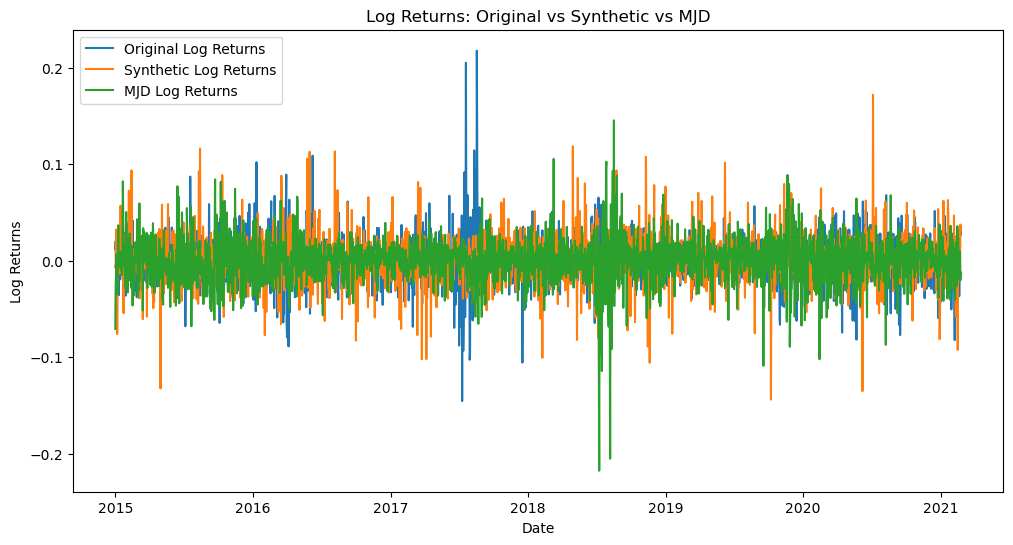
\includegraphics[width=\linewidth]{logreturns.png}
        \caption{Log returns}
        \label{fig:logreturns}
    \end{minipage}
    \hfill
    \begin{minipage}{0.48\textwidth}
        \centering
        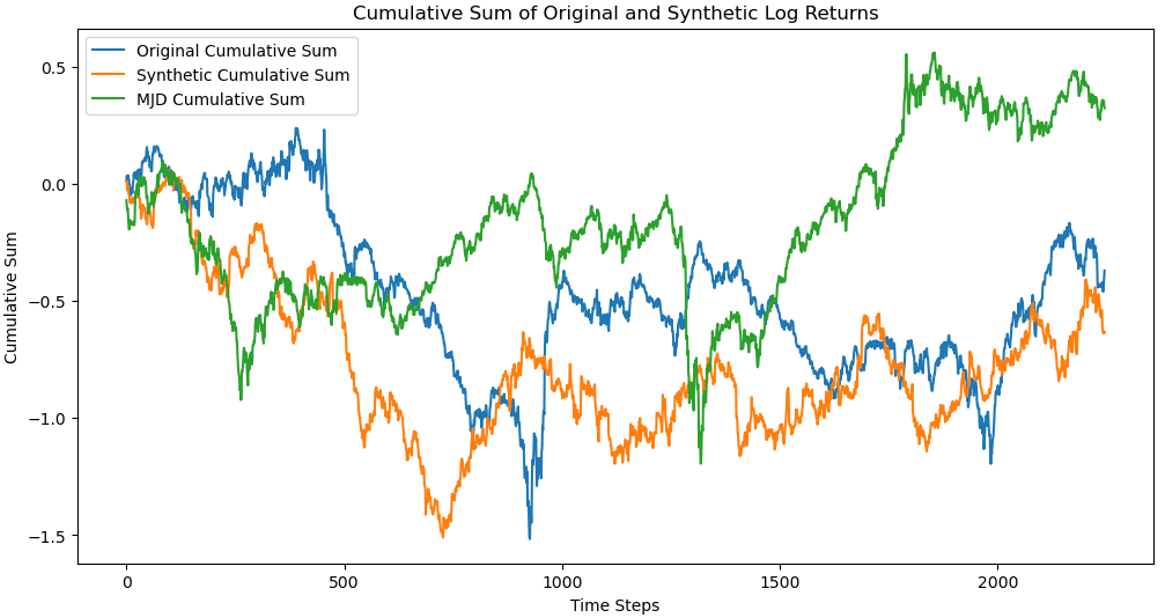
\includegraphics[width=\linewidth]{cumsum.png}
        \caption{Cumulative sum of returns}
        \label{fig:cumsum}
    \end{minipage}
\end{figure}

We can also compare the ACF(Autocorrelation Function) values to see how well the 
QCBM has replicated the structure of the original dataset. ACF aims to quantify 
the correlation between observations separated by a lag value, $k$. This will 
give us insight into market microstructures within the original data as well as 
seeing if the QCBM is able to learn these complexities as well. Formally the ACF 
for a lag $k$ and time series $X$, can be defined as:
\begin{equation}
  \rho_k = \frac{Cov(X_t, X_{t-k})}{\sqrt{Var(X_t)\cdot Var(X_{t-k})}}
\end{equation}
\begin{figure}[h!]
    \centering
    \begin{minipage}{0.48\textwidth}
        \centering
        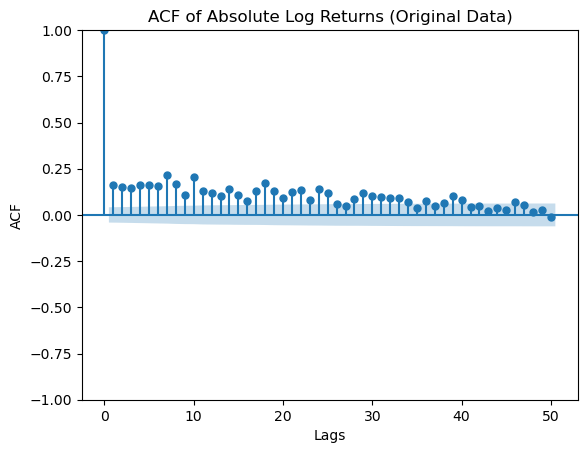
\includegraphics[width=\linewidth]{acfog.png}
        \caption{ACF plot of market data}
        \label{fig:weeklyacfog}
    \end{minipage}
    \hfill
    \begin{minipage}{0.48\textwidth}
        \centering
        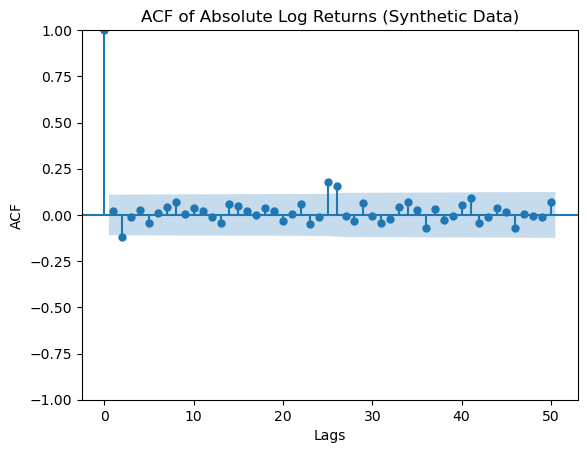
\includegraphics[width=\linewidth]{acfqcbm.png}
        \caption{ACF plot of QCBM data}
        \label{fig:weeklyacfqcbm}
    \end{minipage}
\end{figure}
\begin{figure}[h!]
  \centering
  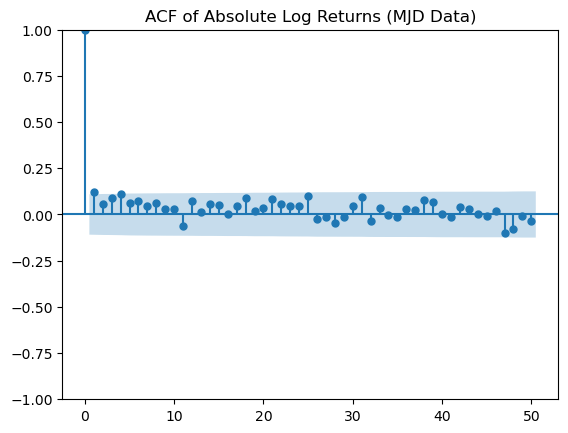
\includegraphics[scale=0.5]{acfmjd.png}
  \caption{ACF plot of MJD data}
  \label{fig:weeklyacfmjd}
\end{figure}
Plots \ref{fig:weeklyacfog} and \ref{fig:weeklyacfqcbm} show the structure of 
the training data vs the QCBM data. The market data shows significant correlation 
between the lags, indicating volatility clustering. This is not reflected in the 
QCBM data, with random spikes showing the model struggles with representing 
volatility persistence. Similar behaviour is observed in the MJD model as shown in 
figure \ref{fig:weeklyacfmjd}. We continue this analysis in further detail in the next section. 
\newpage
\subsection{Volatility Analysis}
It is also important to analyse if the local behaviour of the equity paths is well 
captured. We can do this by analysing the volatility; here the shortfalls of the 
QCBM become clear. Though the global volatility distribution appears to well 
represented, using GARCH models shows a disparity in observed volatility clustering 
compared to the quantum generated volatility. This appears to be a fundamental 
flaw in the model. The assumption that we can represent a path using [give 
equation for propagating path] leads to poor volatility clustering as we have 
treated for each time $0\leq t_0 \leq ...\leq t_n$ our random variable 
$S_{t_r}-S_{t_{r-1}}$ are independent.
\newp 
First looking at rolling volatility, we observe acceptable performance by the 
MJD model, displaying realistic market volatility; the QCBM, however, displayed 
a worse performance, often underestimating volatility peaks, and overestimating 
noise as shown in figure \ref{fig:rollingvol}.
This heightened noise is also reflected 
in figure \ref{fig:weeklyvol} where we see on a weekly basis, the QCBM 
constantly overestimated the volatility. We can observe the difference in learnt 
volatility by comparing distributions. Figure \ref{fig:voldist2} shows us how the 
volatility is skewed with a larger mean and lack of kurtosis. 
\begin{figure}[h!]
    \centering
    \begin{minipage}{0.48\textwidth}
        \centering
        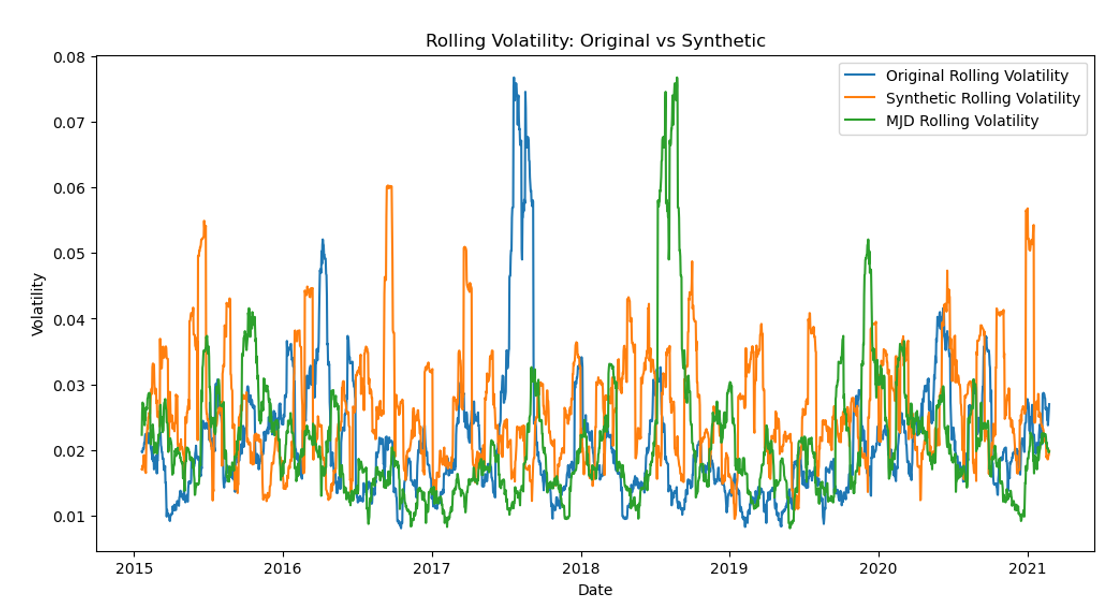
\includegraphics[width=\linewidth]{rollingvol.png}
        \caption{Comparison of rolling volatility (20-day window)}
        \label{fig:rollingvol}
    \end{minipage}
    \hfill
    \begin{minipage}{0.48\textwidth}
        \centering
        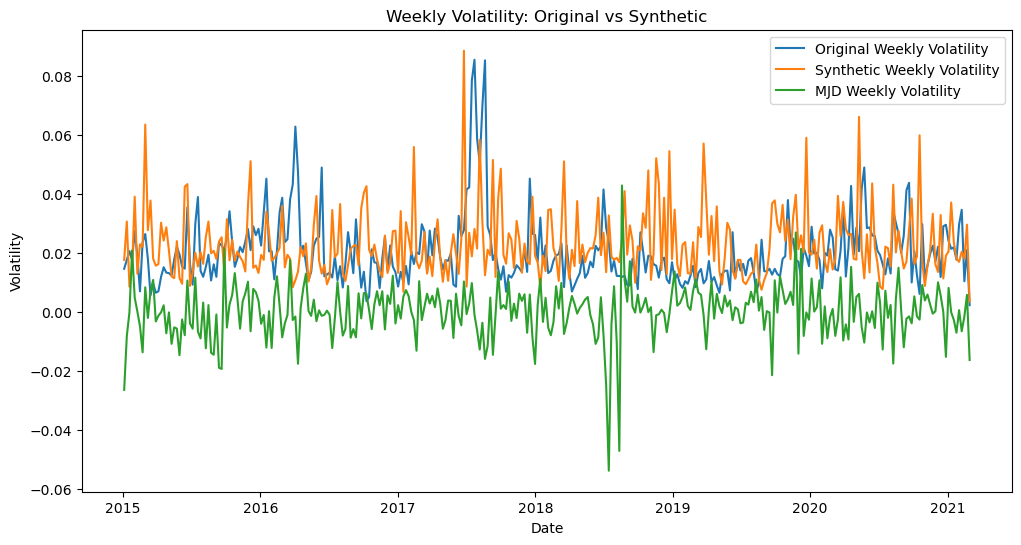
\includegraphics[width=\linewidth]{weeklyvol.png}
        \caption{Comparison of weekly volatility}
        \label{fig:weeklyvol}
    \end{minipage}
\end{figure}
\begin{figure}[h!]
  \centering 
  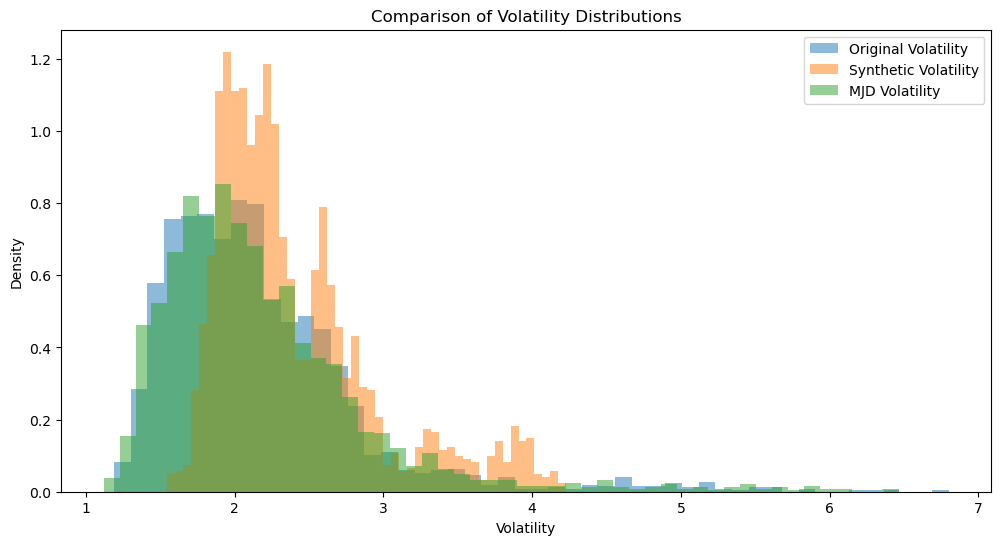
\includegraphics[scale=0.35]{voldist2.png}
  \caption{Comparison of volatility distributions}
  \label{fig:voldist2}
\end{figure}
This story worsens as we look at using volatility models as a comparison method. 
\newp
GARCH (Generalised Autoregressive Conditional Heteroskedasticity) models were 
first introduced in 1982 by Robert Eagle [add reference here] to model volatility 
as a non-constant quantity in financial models. The GARCH(1,1) can be defined as 
so:\\ 
Let $r_t$ be the asset return at time $t$. This can be decomposed as 
\begin{equation}
r_t = \mu + \epsilon_t
\end{equation}
where $\mu$ is the mean return and $\epsilon_t = \sigma_t z_t$ where $z \sim N(0,1)$. 
GARCH models the conditional variance of a given time series process, asset returns in 
our world, as a function of past squared shocks ($\epsilon^2_{t-1}$) and past 
conditional variance ($\sigma^2_{t-1}$). Using this, our model equation becomes
\begin{equation}
  \sigma^2_t = \omega + \alpha\epsilon^2_{t-1} + \beta\sigma^2_{t-1}
\end{equation}
where $\omega > 0$ is the average volatility, $\alpha \geq 0$ is the sensitivity 
to recent shocks, and $\beta \geq0$ is the persistence of volatility, the tendency
of volatility to be high for periods of time and then low of periods of time. 
\newp 
A further model that improved on GARCH is the Exponential GARCH, another model used 
for comparison in my findings. This model focussed on asymmetric volatility 
effects, removing parameter restrictions, and having a logarithmic formulation. 
We can define an EGARCH(1,1) as follows 
\begin{equation}
  \ln(\sigma^2_t) = \omega +\beta\ln(\sigma^2_{t-1})+\gamma\frac{\epsilon_{t-1}}
  {\sigma_{t-1}} + \alpha\Biggl(\frac{|\epsilon_{t-1}|}{\sigma_{t-1}}-\sqrt{\frac{2}{\pi}}\Biggr)
\end{equation}
where the extra term $\gamma$ accounts for the leverage effect; the 
negative correlation between asset returns and volatility change often 
observed in markets.
\newp 
\begin{figure}[h!]
  \centering 
  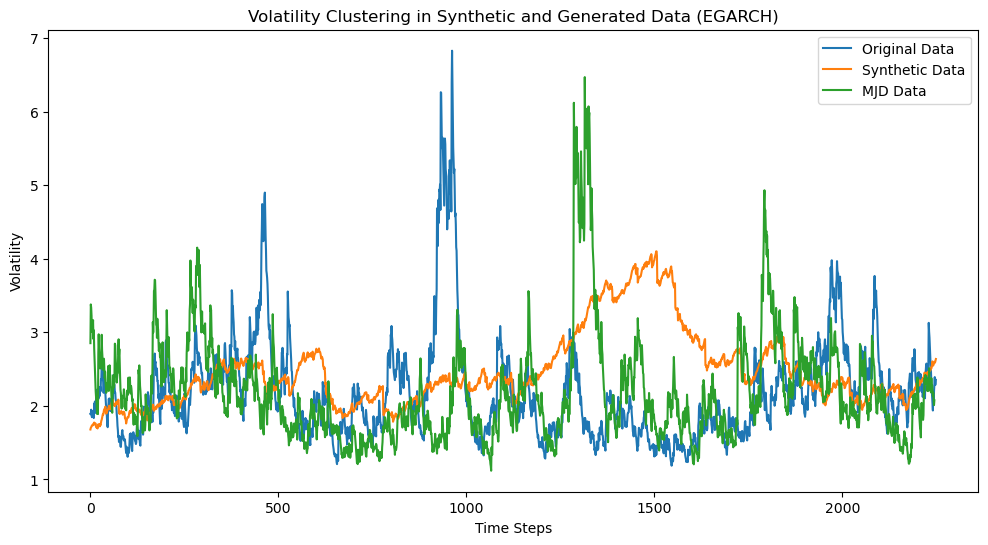
\includegraphics[scale=0.4]{egarch2.png}
  \caption{EGARCH model fit to models}
  \label{fig:egarch2}
\end{figure}
The implementation and parameter estimation for $\omega$,$\alpha$, $\beta$ and 
$\gamma$ were all handled by 
the python package 'arch' [insert this reference https://pypi.org/project/arch/]. 
Calibrating a EGARCH(1,1) to the different model returns gave the following graph. 
In figure \ref{fig:egarch2} we can observe the MJD model displaying more accurate 
clustering compared to the QCBM which remains conservative. This may suggest that 
the MJD model is more suitable for predicting volatility over a short period of 
time. As an improvement to the QCBM, it may be of use to create a hybrid model, 
one that combines the QCBM and a volatility model of choice. 

\newpage
\subsection{VaR \& CVaR}
To determine the usefulness of the generator for hedging purposes, we must explore 
how both generators perform in the extreme percentiles. These are the scenarios 
that we call Black-Swan events; an event that is unexpected, infrequent but has 
huge financial implications. Not being hedged against such changes can leave an 
investor in unwanted positions, exposed to large changes and at risk of losing 
a lot of money. To quantify expected loss a market may give, we employ techniques 
such as VaR(Value at Risk) and CVaR(Conditional Value at Risk). 
\newp 
VaR is a measure that focuses on the loss at a given percentile under normal 
market conditions. It provides a threshold such that the probability of a loss 
exceeding a given value is a chosen percentile i.e 1\% or 5\%. An intuitive 
way to think about it is 1\% VaR of -0.05 means there is a 1\% chance of 
losing at least 5\% of the portfolio value. Mathematically we can define VaR:\\ 
Let $X$ be a random variable with cdf $F_{X}(z)=P\{X\leq z\}$, this is our loss function. 
The VaR of $X$ at a confidence level $\alpha$ is given by
\begin{equation}
  VaR_\alpha(X) = \min\{z|F_X(z)\geq \alpha\}
\end{equation}
VaR, however, has a few crucial limitations. VaR does not say anything about the 
size of losses made after the given $\alpha$ value. This makes it very hard to 
quantify the loss an investor may be exposed to. VaR also assumes liquidity in 
the market at any position when in reality during periods of market stress, the 
ability to buy or sell at any price can be very difficult. It should also be 
known that VaR has a non-subadditivity constraint, meaning VaR for different portfolios 
cannot be added together. For these reasons we opt to use Conditional Value at 
Risk, a more sophisticated tool designed to overcome the given limitations. 
\newp 
CVaR focusses on measuring the risk of extreme losses. Instead of 
considering the probability of losing a given amount, we instead focus on how 
much is lost in the given quantile. This quantifies our tail risk, making it 
appropriate for evaluating the heavy tails of our market generators. Intuitively 
a 1\% CVaR of -0.05 means that, in the worst 1\% of cases, the average loss is 5\%. 
We can define CVaR at a level $\alpha$ as 
\begin{equation}
  CVaR_{\alpha}(X) = \mathbb{E}[X | X \geq VaR_{\alpha}(X)]
\end{equation}
This provides us with a sturdier framework to evaluate performances although we 
must still be careful of its assumptions and limitations. We must assume that the 
distribution of the loss is measured accurately and market conditions are also 
represented faithfully within the given time window. Once we accept these to be 
true, we are provided with a method to compare strategies and generators, as well 
as conforming to financial regulations such as Basel III.
\newp 
The first test was on Eurexx data from the COVID period. This was excluded from the training 
dataset to be used as an extreme market situation. Market generators need to be 
resilient and able to account such market shocks, these are the scenarios where 
hedging positions stop investors from losing large amounts of money.
\begin{table}[h!]
\centering
\begin{tabular}{lcc}
\hline
\textbf{} & \textbf{VaR (1\%)} & \textbf{CVaR (1\%)} \\
\hline
Original Data     & -0.0171 & -0.0174 \\
QCBM Simulated    & -0.0291 & -0.0308 \\
MJDM Simulated    & -0.0360 & -0.0377 \\
\hline
\end{tabular}
\caption{VaR \& CVaR at the 1\% Quantile for COVID data}
\label{tab:cvar_1}
\end{table}
\begin{table}[h!]
\centering
\begin{tabular}{lcc}
\hline
\textbf{} & \textbf{VaR (5\%)} & \textbf{CVaR (5\%)} \\
\hline
Original Data     & -0.0159 & -0.0167 \\
QCBM Simulated    & -0.0223 & -0.0270 \\
MJDM Simulated    & -0.0283 & -0.0338 \\
\hline
\end{tabular}
\caption{VaR \& CVaR at the 5\% Quantile for COVID data}
\label{tab:cvar_5}
\end{table}
At the 1\% quantile we can see both
the MJD and QCBM exhibit greater losses in the tails compared to the real data.
The QCBM has a VaR of 2.91\% and CVaR of 3.08\%, these are both significant 
overestimates of tail risk present in the training data. The MJD overestimates 
the tail risk even greater, expecting much larger than expected losses. We could 
explain this due to the jump component. These pessimistic scenarios, though 
stopping large losses, in reality may lead to over hedging, a situation where a 
given investor may be too protected to the market, limiting potential gains. These 
scenarios may be suboptimal for a deep hedging engine, where the optimal hedge 
is going to be larger than needed. 
\newp 
At the 5\% quantile we see a similar story fold out, both generators estimating 
the tail risk to be greater than observed. The QCBM once again provides a closer 
score to the data, indicating the model is more suitable for hedging purposes, 
though only marginally. What should be noted is the large gap between the VaR 
and CVaR, indicating the MJD model has accounted for significant market shocks,
indicating high sensitivity to extreme events.\\
\newp 
The next scenario is on the unseen continuation of the Brent Crude Oil dataset,
though not excluded purposely than just for out-of-sample testing, the market 
conditions observed have been very volatile. As mentioned earlier, the effect of 
Trump's tariffs were felt in all markets, particularly affecting assets denominated 
in the US dollar. Though as unfortunate as the scenario may be to investors, this 
has provided me with an excellent test for the two models. 
\begin{table}[h!]
\centering
\begin{tabular}{lcc}
\hline
\textbf{} & \textbf{VaR (1\%)} & \textbf{CVaR (1\%)} \\
\hline
Original Data     & -0.0300 & -0.0342 \\
QCBM Simulated    & -0.0429 & -0.0524 \\
MJDM Simulated    & -0.0522 & -0.0631 \\
\hline
\end{tabular}
\caption{VaR \& CVaR at the 1\% Quantile for Brent Crude Data}
\label{tab:cvar_1_brent}
\end{table}

\begin{table}[h!]
\centering
\begin{tabular}{lcc}
\hline
\textbf{} & \textbf{VaR (5\%)} & \textbf{CVaR (5\%)} \\
\hline
Original Data     & -0.0239 & -0.0274 \\
QCBM Simulated    & -0.0313 & -0.0391 \\
MJDM Simulated    & -0.0414 & -0.0508 \\
\hline
\end{tabular}
\caption{VaR \& CVaR at the 5\% Quantile for Brent Crude Data}
\label{tab:cvar_5_brent}
\end{table}
Though the data was more volatile, both models demonstrated that they 
are able to capture the tail risk. The training dataset had large amounts of 
volatility so we would expect good representation of tail risk. 
As seen with the COVID results, 
the models are overestimating the downside risk with scenarios showing 
greater loss than expected. The large gap between the VaR and CVaR values once 
again tells us that the underlying models predict tail events far higher than 
observed in the market. It should be said that the QCBM model is able to reflect 
the tail risk more accurately than the MJD, with value that are closer to the 
original data. One might make conclusions that this makes the QCBM a useful model 
but the poor performance to the original data raises concerns; we can however 
say that the model is more appropriate to use than the MJD in this scenario. 



\subsection{Barren Plateau}
Upon training it was evident that the circuits used: Brick, Butterfly, and Pyramid 
included, all had issues with trainability; the loss function would converge 
at suboptimal parameters. This led me to investigate the loss landscape and reason 
about the difficulties with training the circuit.
\newp 
We first have to confirm whether the barren plateau(BP) is present. As discussed 
earlier, BP occurs when the gradient of the cost function with respect to the 
parameters, $\frac{\partial C}{\partial \theta}$, tends to 0. Plotting this gave
us results that were unexpected. Figure \ref{fig:gradvar} shows us that the 
variance of the gradient increases as we increase the qubit count, going against 
what the maths would suggest. One theory was that the nature of the data led to 
such phenomenon. 
\newp
To confirm such beliefs, I used the QCBM to learn several distributions. These 
included:
\begin{itemize}
  \item Step function: $H(x) = \begin{cases} 
                                0 & \text{if } x < 0, \\
                                1 & \text{if } x \geq 0 
                              \end{cases}$
  
  \item Dirac delta function: $\delta(x) = \begin{cases} 
                                          \infty & \text{if } x = 0, \\
                                          0 & \text{otherwise}
                                        \end{cases}$ with $\int_{-\infty}^{\infty} \delta(x) \, dx = 1$
  
  \item Uniform distribution: $U(x; a, b) = \begin{cases} 
                                          \frac{1}{b-a} & \text{if } a \leq x \leq b, \\
                                          0 & \text{otherwise}
                                        \end{cases}$
  
  \item Normal distribution: $\mathcal{N}(x; \mu, \sigma^2) = \frac{1}{\sigma\sqrt{2\pi}} e^{-\frac{(x-\mu)^2}{2\sigma^2}}$

\end{itemize}
\begin{figure}[h!]
    \centering
    \begin{minipage}{0.48\textwidth}
        \centering
        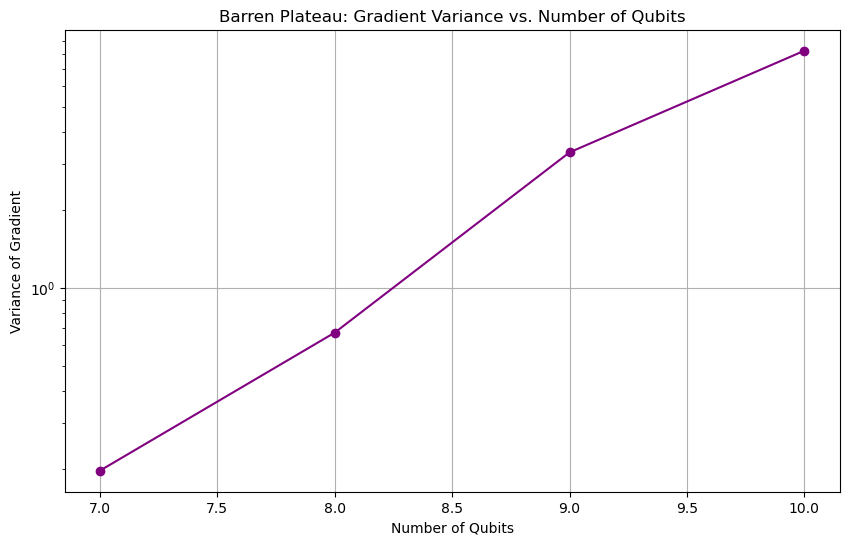
\includegraphics[width=\linewidth]{gradvar.png}
        \caption{Variance of the gradient vs qubit count}
        \label{fig:gradvar}
    \end{minipage}
    \hfill
    \begin{minipage}{0.48\textwidth}
        \centering
        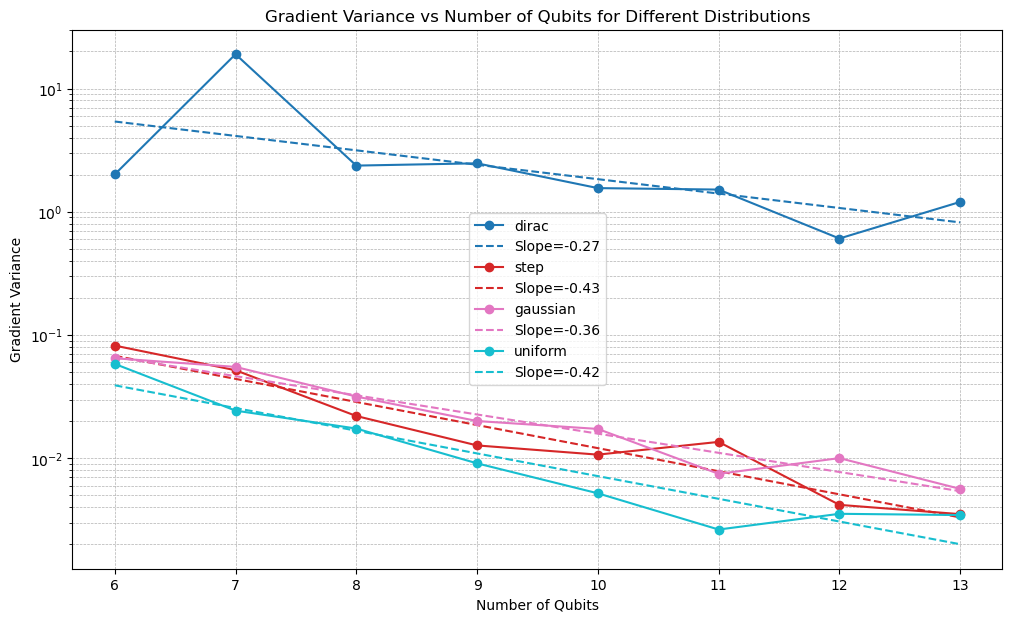
\includegraphics[width=\linewidth]{bpmultipledists.png}
        \caption{Variance of gradients vs qubit count for multiple distributions}
        \label{fig:bpmultiple}
    \end{minipage}
\end{figure}
What is intriguing is how the dirac function performed. This suggested spikes in 
the data had an impact on the trainability, to further reinforce this point I 
tested how the QCBM performed with a function that contains many spikes. 
\begin{figure}[h!]
    \centering
    \begin{minipage}{0.48\textwidth}
        \centering
        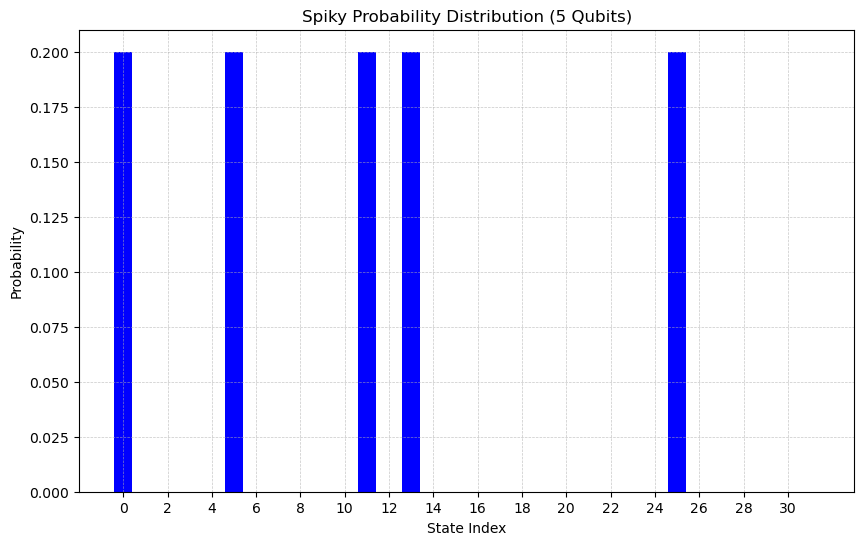
\includegraphics[width=\linewidth]{mdiracgraph.png}
        \caption{Spiky distribution}
        \label{fig:mdirac}
    \end{minipage}
    \hfill
    \begin{minipage}{0.48\textwidth}
        \centering
        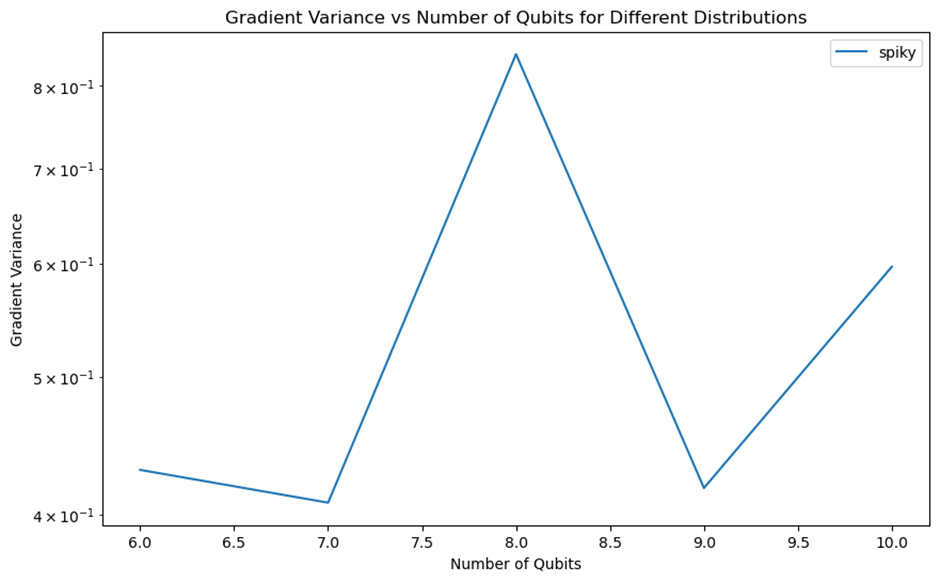
\includegraphics[width=\linewidth]{mdiracbp.png}
        \caption{Variance of gradients vs qubit count for a spiky distribution}
        \label{fig:bpdirac}
    \end{minipage}
\end{figure}
Figures \ref{fig:mdirac} \& \ref{fig:bpdirac} show the distribution learnt and 
how the variance of the cost gradients change. The spiky nature of the plot 
indicates that there is something else affecting the QCBM's performance beyond 
just barren plateau. This effect was beyond the scope of this report but can be 
investigated after this project. 
\subsubsection{ZX Calculus}
Reducing the T-gate count was essential to improve the trainability. 
I first plotted the loss landscape for some of the gate combinations to visualise 
how the loss changes with different gate pairs. As shown in the graphs, the 
optimisation process for the first layers is much simpler to converge than for 
the latter gates. The local minimas presented in comparing layers 4 and 6 
demonstrates the need to reduce gate count to simplify the optimisation process. 
\begin{figure}[h!]
    \centering
    \begin{minipage}{0.48\textwidth}
        \centering
        \includegraphics[width=\linewidth]{landscape1.png}
        \caption{Loss landscape for gates in the first 2 layers}
        \label{fig:landscape1}
    \end{minipage}
    \hfill
    \begin{minipage}{0.48\textwidth}
        \centering
        \includegraphics[width=\linewidth]{landscape2.png}
        \caption{Loss landscape for gates at an increased depth}
        \label{fig:landscape2}
    \end{minipage}
\end{figure}

\newpage 
\section{Project Management}

\newpage
\section{Outlook and Conclusions}
This project was designed to investigate the quantum advantages as compared to 
traditional techniques for deep hedging, and all the goals set out have been 
fulfilled. Through thorough analysis of model performances, I am able to say that 
the QCBM outperformed the Merton-Jump Diffusion model in modelling the fat tails 
and skewness of the market data. 
\newp
In the context of hedging, the synthetic data generated would most likely not be 
acceptable as the lack of volatility clustering may lead to suboptimal hedges 
in the hedging engine. The overestimation of tail risk was also prevalent, possibly 
leading to an over-hedge, minimising the potential upside of a trade. It should 
also be said, while talking to oil traders, it came up that traders would often 
under hedge their positions. This is due to the fact they are placing a directional 
bet based on their reasoning, be it mathematical or due to experience. 
This is a factor that is not considered but should be thought about when designing
a hedging engine. This further emphasising the point that though the QCBM appears 
superior in the chosen metrics, it may not be completely suitable for a hedging 
engine. For further analysis, comparisons against machine learning techniques
can be executed, deducing whether this method beats all methods of simulation on 
classical devices. 
\newp 
I also explored issues with trainability, coming across a phenomenon where the 
variance of the cost gradient increased, or appeared uncorrelated when dealing 
with distributions with scattered high densities. Beyond this research, I would like 
to explore this, mathematically reasoning the effect and mitigation techniques. 
\newp 
Optimisation techniques such as T-gate reduction using ZX calculus was also 
explored, showing the strength of such representation. I believe this another 
area of research that can be extended beyond this project, investigating 
different gate reduction techniques, ones perhaps that may be better suited for 
this nature of data. 
\newp
There is new research being done on Quantum Monte Carlo techniques, boasting
superiority over classical quasi-monte carlo methods due to the truly random 
nature of quantum mechanics. Moving beyond this paper, this technique can be 
added easily to the current framework for simulation of asset prices and 
deep hedging. 
\newp
This technique of generating synthetic data has applications beyond deep hedging 
and quantitative finance. The framework set up can be adapted for use cases where 
lack of training data is present, or for scenarios where the underlying distribution 
is difficult to learn classically. 

\clearpage
\section{Appendix}
\subsection{QCBM Architectures}

\begin{figure}[h!]
    \centering
    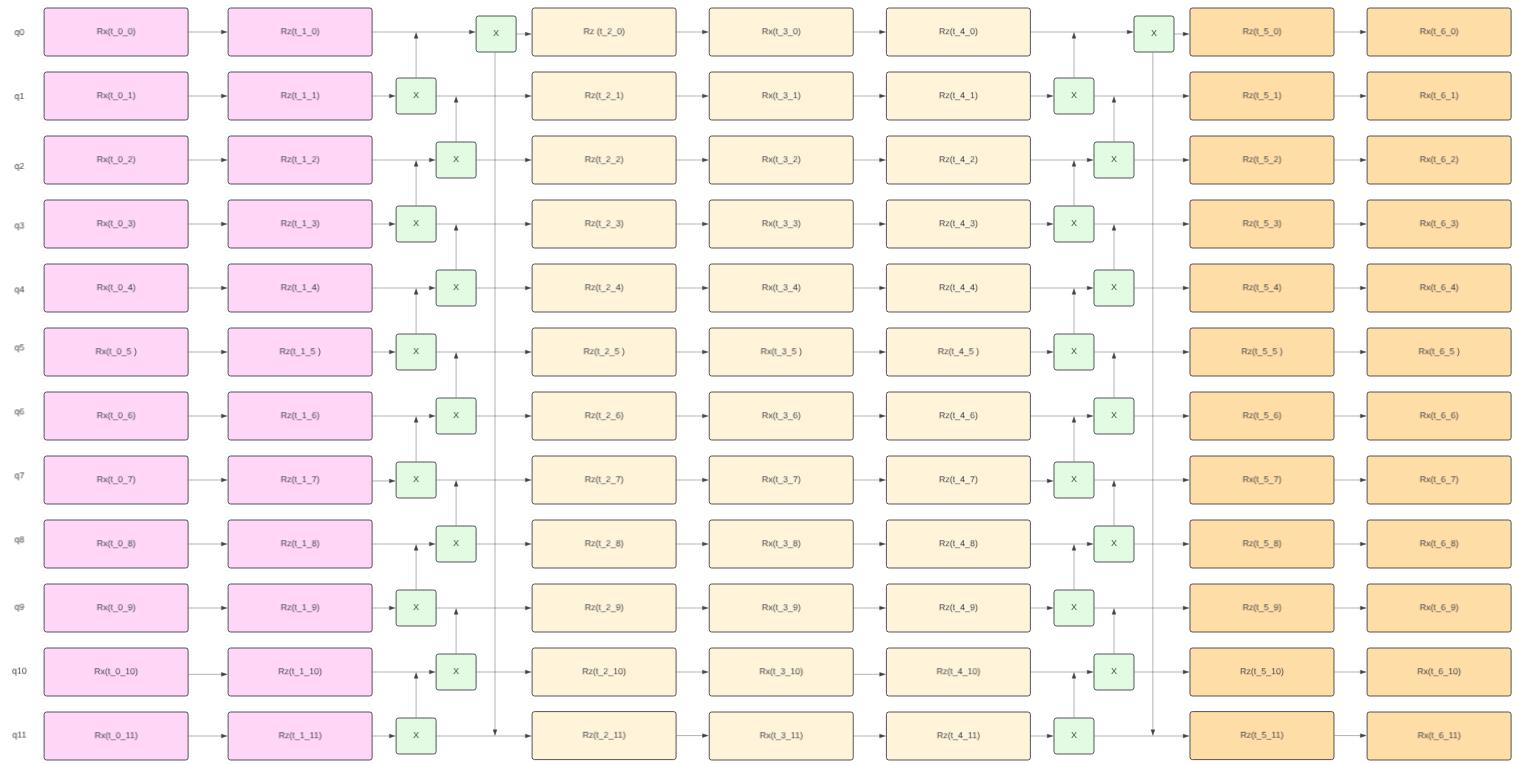
\includegraphics[scale=0.3, angle=270, width=\textwidth-209]{qcbm1.png}
    \caption{QCBM architecture}
\end{figure}
\clearpage


\printbibliography

\end{document}

